%% -*- TeX-engine: xetex; ispell-dictionary: "russian" -*-

\documentclass[a4paper,14pt]{au-diploma}

\usepackage{microtype}

\usepackage{chemfig}

\usepackage{fancyvrb}
\newcommand{\bl}[1]{\textbf{#1}}

%% Устраняет проблемы с переносом слов, содержаших дефис.
\usepackage{hyphenat}

%% Библиография.
\usepackage{csquotes}
\usepackage[style=gost-numeric-min,backend=biber,movenames=false]{biblatex}
\addbibresource{references.bib}

%% Plate notation.
\usepackage{tikz}

\usetikzlibrary{arrows,calc,shapes,positioning}
\usetikzlibrary{bayesnet}

%% Total pages, figures etc.
\usepackage[figure,page,table]{totalcount}

%% Caption hacking.
\usepackage{subcaption}
\renewcommand{\thesubfigure}{\asbuk{subfigure}}
\renewcommand{\thesubtable}{\asbuk{subtable}}
\usepackage[font=small,tableposition=top,margin=1em]{caption}

%% Float barriers.
\usepackage{placeins}

%% Line break after paragraph title.
\makeatletter
\renewcommand\paragraph{\@startsection{paragraph}{4}{\z@}%
  {-3.25ex\@plus -1ex \@minus -.2ex}%
  {1.5ex \@plus .2ex}%
  {\normalfont\normalsize\bfseries}}
\makeatother

\DeclareMathOperator*{\argmin}{arg\,min}
\DeclareMathOperator*{\argmax}{arg\,max}
\newcommand{\E}[2]{\mathbb{E}_{#1} \left[ #2 \right]}
\newcommand{\I}[1]{\mathbb{I}\left( #1 \right)}
\newcommand{\op}[1]{\operatorname{#1}}

\sloppy  %% Awww...

\begin{document}

%% -*- TeX-engine: xetex; TeX-master: "draft.tex"; ispell-dictionary: "russian" -*-

\begin{titlepage}
  \thispagestyle{empty}

  \begin{center}
    
\includegraphics[width=\textwidth]{images/au}
  \end{center}

  \small

  \begin{flushright}
    \begin{minipage}[t]{0.4\textwidth}%
      \begin{center}
        На правах рукописи

        \par\bigskip

        Диссертация допущена к защите\\
        Зав. кафедрой\\
        Омельченко А.В.
        \underline{\hspace{6cm}}
       <<\underline{\hspace{0.5cm}}>> \underline{\hspace{3cm}} 2014 г.
      \end{center}
    \end{minipage}
  \end{flushright}

  \par\bigskip
  \par\bigskip
  \par\bigskip
  \par\bigskip

  \begin{center}
    \textbf{\uppercase{Д И С С Е Р Т А Ц И Я}}\\
    \uppercase{НА СОИСКАНИЕ УЧЕНОЙ СТЕПЕНИ}\\
    \textbf{\uppercase{М А Г И С Т Р А}}

  \end{center}

  \par\bigskip
  \par\bigskip

  Тема:  Моделирование данных бисульфитного секвенирования

  \par\bigskip
  \par\bigskip

  Направление: \hfill 010900.68 --- Прикладные математика и физика

  \par\bigskip
  \par\bigskip

  Выполнил студент \hfill С.А. Лебедев

  {\scriptsize
    \begin{center}
      (подпись)
    \end{center}
  }

  Руководитель \hfill О.Ю. Шпынов

  {\scriptsize н. с.
    \begin{center}
      (подпись)
    \end{center}
  }

  \par\bigskip

  Рецензент \hfill С.В. Малов

  {\scriptsize ведущий н.с., доцент, к.ф.-м.н.
    \begin{center}
      (подпись)
    \end{center}
  }

  \vfill

  \begin{center}
    Санкт-Петербург

    2014 г.
  \end{center}

  \normalsize

  \newpage
\end{titlepage}


%% -*- TeX-engine: xetex; TeX-master: "draft.tex"; ispell-dictionary: "russian" -*-

\thispagestyle{empty}

\addtocontents{toc}{\protect\setcounter{tocdepth}{0}}
\section*{Реферат}

С.~\totalpages, рис.~\totalfigures, табл.~\totaltables.

В данной работе представлена вероятностная модель для анализа результатов
бисульфитного секвенирования. Предлагаемая модель является расширением
класса скрытых марковских моделей и называется переключающейся мультиномиальной
скрытой марковской моделью. У модели три состояния: одно из состояний соответствует
ошибкам бисульфитной конверсии, а другие два позволяют отличать области гиперметилирования
от областей гипометилирования. Модель предполагает, что вероятность перехода между
состояниями зависит от расстояния между моделируемыми наблюдениям. Использование
мультиномиального распределения для моделирования информации о покрытии
цитозинов позволяет учитывать наличие ошибок секвенирования. Реализация
модели была выполнена на языке Java в рамках биоинформатического проекта компании
JetBrains.

\textbf{Ключевые слова}: вероятностная модель, скрытая марковская модель,
эпигенетика, метилирование ДНК, бисульфитное секвенирование.

\addtocontents{toc}{\protect\setcounter{tocdepth}{2}}


%% Первая страница --- титульный лист.
\setcounter{page}{2}
\tableofcontents

%% -*- TeX-engine: xetex; TeX-master: "draft.tex"; ispell-dictionary: "russian" -*-

\section*{Введение}

ДНК (дезоксирибонуклеиновая кислота) --- длинная двухцепочечная молекула, являющаяся носителем
генетической информации в биологических организмах. Совокупность ДНК биологического организма
называют геномом. Основу цепочки ДНК составляют четыре нуклеотидных остатка: аденин, гуанин, цитозин и
тимин.

% TODO: эпигенетика
% С нуклеотидами в составе молекулы ДНК могут происходить генетические и эпигенетические
% изменения. Первая группа включает в себя изменения которые изменяют последовательность нуклеотидов
% в цепочке, например, замена одного нуклеотида на другой или удаление нуклеотида. Изменения во второй
% группе не изменяют структуру ДНК.

Присоединение метильной группы ($\op{CH}_3$) к цитозину в составе молекулы ДНК является
одним из ключевых механизмов регуляции жизни клетки \cite{Smith2013}. Это и есть
метилирование ДНК. Одним из методов экспериментальной оценки метилирования является
бисульфитное секвенирование. Суть метода заключается в обработке ДНК бисульфитом натрия с
последующим секвенированием, то есть чтением нуклеотидной последовательности.

Мотивацией для анализа метилирования послужили исследования
\cite{lister2009human,Stadler2011,Xie2013}, авторы которых изучали данные бисульфитного
секвенирования человека и мыши и пришли к выводу, что области генома, редко содержащие
цитозины с метильной группой, представляют особый интерес для изучения. В частности,
в работе \cite{Stadler2011} было показано, что области гипометилирования\footnote{
Цитозин называется \emph{гипометилированым}, если к нему редко присоединяется метильная группа.
Обратная ситуация называется \emph{гиперметилированием}, в этом случае метильная группа почти
всегда присутствует.} находятся в похожем состоянии у различных видов, а также оказывают
влияние на находящиеся рядом функциональные участки генома. Изменение метилирования
влияет на эти участки, тем самым вызывая нарушения в жизнедеятельности клетки, например,
приводя к раку \cite{Xie2013}.

Для получения информации о строении и внутренних процессах клетки ставятся
биологические эксперименты, например, бисульфитное секвенирование. Во время
этих экспериментов мы не можем обеспечить изоляцию от окружающей среды, а
также идеальную точность измерительных приборов. Из-за этого в результатах
экспериментов появляется шум, и последующий анализ получается неточным. Частично
эту проблему решает использование вероятностных моделей. Возвращаясь к бисульфитному
секвенированию, можно отметить, что моделей для него почти нет, а существующие,
скорее всего, можно улучшить.

Цель данной работы --- разработать математическую модель, позволяющую качественно
описывать результаты бисульфитного секвенирования.

Для достижения цели были поставлены следующие задачи.

\begin{enumerate}
\item Проанализировать существующие подходы к обработке и моделированию данных бисульфитного
  секвенирования.
\item Предложить, обосновать и реализовать несколько вероятностных моделей.
\item Сформулировать критерии отбора и выбрать наиболее подходящую модель.
\item Сравнить выбранную модель с уже существующими.
\end{enumerate}

%% -*- TeX-engine: xetex; TeX-master: "draft.tex"; ispell-dictionary: "russian" -*-

\section{Обзор задачи}

\subsection{Биологические сведения}

\subsubsection{Метилирование ДНК}

Метилирование ДНК --- модификация цитозина в составе молекулы
ДНК, заключающаяся в присоединении метильной группы к C5-позиции цитозинового кольца
(рис.~\ref{fig:methylation}). Несмотря на то, что это не структурное изменение, при
делении клетки оно может сохраняться~\cite{Jones2012}.

\begin{figure}[h]
  \begin{center}
    \begingroup
    \setatomsep{1.8em}
    \chemname[1.8em]{\chemfig[line width=1pt]{*6([,,1]-\chembelow{N}{H}-(=O)-N=(-NH_2)-=)}}{цитозин}
    \setchemrel{1pt}{0pt}{8.5em}
    \chemrel{->,thick}
    \chemname[1.8em]{\chemfig[line width=1pt]{*6([,,1]-\chembelow{N}{H}-(=O)-N=(-NH_2)-(-CH_3)=)}}{5-метилцитозин}
    \endgroup
  \end{center}
  \caption{Метилирование ДНК}
  \label{fig:methylation}
\end{figure}

\subsubsection{Бисульфитное секвенирование}

Метилирование ДНК относится к классу эпигенетических модификаций, так как при присоединении метильной
группы к цитозину нуклеотидная структура ДНК не изменяется. Это обстоятельство мешает использовать
существующие методы анализа нуклеотидной последовательности для анализа метилирования. Решить
проблему можно с помощью химического механизма \emph{бисульфитной конверсии}, который позволяет
закодировать информацию о статусе метилирования в структуре ДНК. Суть механизма заключается в
следующем: под действием бисульфита натрия цитозин без метильной группы конвертируется в урацил;
5\hyp метилцитозин при этом не конвертируется.

Существуют различные методы анализа обработанной бисульфитом натрия ДНК \cite{Jones2012}, например,
полимеразная цепная реакция (ПЦР), ДНК\hyp микрочипы или секвенирование. Последний метод, называемый
\emph{бисульфитным секвенированием}, позволяет получить информацию о статусе метилирования каждого
цитозина в геноме, поэтому для полногеномного анализа метилирования используют именно его
\cite{lister2009human,Stadler2011,Xie2013,Ziller2013}.

В ходе секвенирования случайные фрагменты ДНК, обработанной бисульфитом натрия, читаются
секвенатором в объёме, достаточном для того, чтобы с большой вероятностью каждый
фрагмент был прочитан несколько раз. При этом урацил будет прочитан секвенатором как
тимин, а 5-метилцитозин --- как цитозин. Затем для каждого полученного прочтения ищется
соответствующий ему участок последовательности генома (рис.~\ref{fig:bsseq}). Обычно прочтения,
которым может соответствовать более одного участка в геноме, исключают из рассмотрения.

\begin{figure}[h]
  \centering
\begin{Verbatim}[commandchars=\\\{\}]
                 ↓            ↓      ↓
          CAAAAGA\bl{C}AAATAGTGATGT\bl{C}ACCAAT\bl{C}GAGC
          --------------------------------
               GA\bl{C}A         GT\bl{C}A  AAT\bl{T}
              AGA\bl{T}         TGT\bl{C}
               GA\bl{C}A   AGTG TGT\bl{C}    AT\bl{T}G
\end{Verbatim}
  \caption{Схематическое изображение выравнивания прочтений секвенатора (под чертой)
    на известную последовательность генома (над чертой). Стрелка (\texttt{↓}) указывает на
    метилированный цитозин.}
  \label{fig:bsseq}
\end{figure}

В качестве характеристики статуса метилирования конкретного цитозина в геноме обычно
используют \emph{уровень метилирования} ${\beta = \frac{\#C}{\#C + \#T} \in [0, 1]}$, где $\#C$ ---
количество прочтений, подтверждающих наличие метилирования, а $\#T$ --- количество прочтений,
опровергающих его. Можно считать, что $\beta$ --- оценка вероятности того, что случайно
взятое прочтение, покрывающее рассматриваемый цитозин, будет подтверждать метилирование.

Иногда вместо уровня метилирования также используют пару $(\#C, \#T)$ без каких-либо преобразований.

Протокол бисульфитного секвенирования, как уже было сказано, не исключает наличие в результатах
эксперимента ошибок. Кратко перечислим их основные источники.

\begin{itemize}
\item Недостаточная или избыточная обработка ДНК бисульфитом натрия приводит к
  ошибкам бисульфитной конверсии \cite{pmid18984622}, то есть переходам вида
  (цитозин $\rightarrow$ цитозин) и (5-метилцитозин $\rightarrow$ урацил).
\item Точечная мутация (цитозин $\rightarrow$ тимин) может ошибочно подтверждать наличие
  метилирования.
\item Ошибки секвенирования \cite{pmid22067484}, то есть неправильные прочтения секвенатором
  фрагментов ДНК, касающиеся цитозина и тимина, влияют на получаемые значения $\#C$ и $\#T$.
\end{itemize}

\subsection{Статистические сведения}

\subsubsection{Встречающиеся распределения}
\label{subsub:mentioned}

В тексте работы встречаются некоторые известные \cite{murphy2012machine} распределения. Ниже
приведены их функции плотности вероятности или функции вероятности в зависимости от области
определения.
\begin{itemize}
\item Биномиальное распределение:
  $$
  \op{Bin}(k; n, p) = \binom{n}{k} p^k (1 - p)^{n - k}
  \quad k \in \{0, \ldots, n\}; n \in \mathbb{N}_0, p \in [0, 1].
  $$
\item Мультиномиальное распределение:
  \begin{align*}
    \op{Mult}(\mathbf{k}; n, \mathbf{p})
    = \I{\sum_{i = 1}^d k_i = n} \frac{n!}{k_1! \dots k_d!} p_1^{k_1} \dots p_d^{k_d} \\
    k_i \in \{0, \ldots, n\}; n \in \mathbb{N}, p_i \in [0, 1], \sum\limits_{i = 1}^d p_i = 1,
  \end{align*}
  где $\I{x}$ --- индикаторная функция.
\item Дискретное (категориальное) распределение:
  $$
  \op{Cat}(k; \mathbf{p}) = p_1^{\I{k = 1}} \dots p_d^{\I{k = d}}
  \quad k \in \{1, \ldots, d\}; p_i \in [0, 1], \sum\limits_{i = 1}^d p_i = 1.
  $$
\item Распределение Гаусса (нормальное):
  $$
  \op{N}(x; \mu, \sigma^2)
  = \frac{1}{\sigma \sqrt{2 \pi}} \exp \left( - \frac{(x - \mu)^2}{2 \sigma^2} \right)
  \quad x \in \mathbb{R}; \mu \in \mathbb{R}, \sigma \in \mathbb{R}_{> 0}.
  $$
\item Бета-биномиальное распределение:
  \begin{align*}
  \op{BetaBin}(k; n, \alpha, \beta)
  = \binom{n}{k} \frac{\op{B}(k + \alpha, n - k + \beta)}{\op{B}(\alpha, \beta)} \\
  k \in \{0, \ldots, n\}; n \in \mathbb{N}_0, \alpha, \beta \in \mathbb{R}_{> 0}.
  \end{align*}
  Если $\alpha = \beta$, то распределение называется симметричным бета\hyp биномиальным.
\end{itemize}

\subsubsection{Математическое ожидание}

В работе используются следующие обозначения, связанные с математическим ожиданием.

\begin{itemize}
\item Математическое ожидание:
  $$
  \E{X}{f(X)} = \int f(x) p(x) dx,
  $$
  где $p(x)$ --- плотность распределения случайной величины $X$.
\item Условное математическое ожидание:
  $$
  \E{X|Y = y}{f(X)} = \int f(x) p(x|Y = y) dx,
  $$
  где $p(x|Y = y)$ -- плотность распределения случайной величины $X$ при
  условии того, что случайная величина $Y$ принимает значение $y$. В случаях, где это
  непротиворечиво, мы будем писать $\E{X|y}{f(X)}$ вместо $\E{X|Y = y}{f(X)}$.
\end{itemize}

\subsubsection{Информационный критерий Акаике}

Информационный критерий Акаике применяется для выбора из нескольких моделей, обученных на
одних и тех же данных методом максимального правдоподобия. Значение критерия для конкретной
модели вычисляется по формуле
$$
\op{AIC} = 2k - 2 \log L,
$$
где $k$ --- число параметров модели, а $L$ --- правдоподобие данных с точки зрения модели.
Критерий Акаике позволяет отранжировать модели по относительной предпочтительности: чем
ниже вычисленная величина, тем лучше модель. Критерий Акаике штрафует модели с большим
количеством параметров и тем самым защищает от переобучения \cite[С. 163-164]{murphy2012machine}.

\subsection{Существующие подходы}
\label{sub:existing}

\subsubsection{Скрытая марковская модель с Гауссовыми испусканиями}

Авторы \cite{Stadler2011} предлагают моделировать уровни метилирования с помощью скрытой
марковской модели \cite{Rabiner1989} с тремя состояниями: одно из состояний соответствует
ошибкам бисульфитной конверсии, а другие два позволяют отличать области гиперметилирования
от областей гипометилирования. Значение уровня метилирования моделируется с помощью распределения
Гаусса (см.~\ref{subsub:mentioned}). Обучение модели производится методом максимального
правдоподобия.

\paragraph{Анализ подхода}

Моделирование уровня метилирования, а не пары $(\#C, \#T)$, накладывает ограничения на
чувствительность модели, например, уровни метилирования $^5/_{10}$ и $^1/_2$ для модели
идентичны. Стоит также заметить, что распределение Гаусса определено на $\mathbb{R}$,
в то время как уровень метилирования --- величина из $[0, 1]$, то есть предлагаемая
авторами модель не соответствует моделируемым данным.

\subsubsection{MethylSeekR}

Одной из особенностей \cite{lister2009human,gaidatzis2014} метилирования в человеке является наличие
частично метилированных участков (partially methylated domains, PMDs)~---~длинных областей генома, в
которых распределение уровней метилирования стремится к равномерному. Авторы работы
\cite{Burger2013} предлагают трёхшаговую процедуру для нахождения регуляторных областей
гипометилирования в данных бисульфитного секвенирования человека с учётом наличия PMD.
Для этого геном сначала разбивается на непересекающиеся участки, содержащие 101
цитозин. Пары $(\#C, \#T)$ внутри одного участка моделируются с помощью симметричного
бета-биномиального распределения (см.~\ref{subsub:mentioned}), описываемого параметром
$\alpha$. Значение параметра $\alpha$ находится как апостериорное среднее. Вторым шагом
авторы предлагают моделировать последовательность $\alpha$ скрытой марковской моделью с
Гауссовыми испусканиями и двумя состояниями: участок является PMD или не является PMD.
Найденные таким образом частично метилированные участки исключаются из рассмотрения.
Гипометилированные области находятся среди оставшихся участков с помощью отсечки на уровень
метилирования, которая выбирается с помощью рандомизированной процедуры.

\paragraph{Анализ подхода}

Авторы не приводят мотивацию для выбора размера моделируемого участка, а также не
исследуют чувствительность метода к его размеру. Предположительно, с увеличением
размера участка распределение уровней метилирования будет стремиться к равномерному,
то есть $\alpha \approx 1$, что снизит чувствительность шага фильтрации PMD.

Аналогично предыдущему подходу, авторы используют распределение Гаусса для моделирования
положительной величины.

\subsubsection{MSC}
\label{subsub:msc}

В работе \cite{Cheng2014} предлагается алгоритм, позволяющий с некоторым ограниченным количеством
ошибок отделить цитозины без метильной группы от 5-метилцитозинов. Алгоритм основан на использовании
биномиальной смеси с двумя состояниями для моделирования пар $(\#C, \#T)$. Параметры смеси
оцениваются методом максимального правдоподобия.

\paragraph{Анализ подхода}

Основным результатом этой работы является использование подходов из теории кластерного
анализа и статистической проверки гипотез для контроля количества ошибок первого рода
(цитозин ошибочно назван метилированным) в результатах биномиальной смеси.

\subsection{Экспериментальные данные}
\label{sub:data}

NCBI GEO\footnote{\url{http://www.ncbi.nlm.nih.gov/geo}} --- крупнейший открытый архив экспериментальных
данных, полученных из биологических экспериментов. Эксперименты внутри NCBI GEO объединены в серии. У
каждой серии экспериментов есть свой уникальный номер, по которому можно найти описание протокола,
использованного для получения данных, последовательность этапов пост-обработки данных,
названия связанных статей и так далее.

Для оценки моделей в данной работе используются данные бисульфитного секвенирования стволовых клеток
мыши (\emph{M. musculus}), описанные в статье \cite{Stadler2011}, номер серии экспериментов GSE30202.

%% -*- TeX-engine: xetex; TeX-master: "draft.tex"; ispell-dictionary: "russian" -*-

\section{Предлагаемые модели}
\label{sec:models}

\subsection{Конкретизация задачи}

Пусть $\mathbf{x} = (x_1, \ldots, x_T)$ --- некоторое представление результатов
бисульфитного секвенирования, где $t$-му цитозину соответствует наблюдение $x_t$.
Мы будем предполагать, что каждому наблюдению $x_t$ можно сопоставить некоторую
метку-состояние $s_t$ из множества состояний $\{1, \ldots, S\}$. Истинные значения
$s_t$ нам не известны. Вероятностная модель позволяет найти наиболее правдоподобную
(в смысле модели) последовательность состояний:
$$
\hat{\mathbf{s}}_{ML}
= \argmax\limits_{\mathbf{s} \in \{1, \ldots, S\}^T} P(\mathbf{x}, \mathbf{s}|\mathbf{\theta}),
$$
где $\mathbf{\theta}$ --- вектор параметров модели.

В данной работе используется множество состояний, предложенное в \cite{Stadler2011}:
состояние $1$ или \texttt{UNMETHYLATED} соответствует ошибкам бисульфитной конверсии,
$2$ или \texttt{LOW} --- областям гипометилирования, а $3$ или \texttt{HIGH} ---
областям гиперметилирования.

\subsection{Биномиальная смесь}

\subsubsection{Мотивация}

Пусть $x_t = (k_t, n_t)$ --- количество прочтений, подтверждающих метилирование,
и общее количество прочтений для $t$-го цитозина. При построении самой простой модели
предполагается, что состояния всех наблюдений независимы и одинаково распределены,
а также, что $k_t$ подчиняются биномиальному распределению с параметрами $n_t$ и $p_{s_t}$,
где $p_{s_t}$ --- вероятность того, что прочтение подтверждает метилирование цитозина.
Такое предположение соответствует смеси $S$ биномиальных распределений. Распределения,
образующие смесь, называются \emph{компонентами} смеси.

\subsubsection{Определение}
Пусть $\mathbf{\pi} = (\pi_1, \ldots, \pi_S)$ --- априорные вероятности компонент смеси
и $\mathbf{p} = (p_1, \ldots, p_S)$ --- параметры биномиального распределения для каждой
из компонент, причём
$$
\sum\limits_{i = 1}^S \pi_i = 1,
$$
тогда правдоподобие данных при условии модели
$$
P(\mathbf{k}; \mathbf{n}, \mathbf{\pi}, \mathbf{p})
= \prod\limits_{t = 1}^T \sum\limits_{i = 1}^S
  \pi_i \op{Bin}(k_t; n_t, p_i)
$$

Для модели можно также сформулировать порождающий процесс, то есть описание того,
как с её помощью можно получить наблюдаемую выборку: для каждого $t$-го наблюдения
выберем скрытое состояние $s_t$ из дискретного распределения с параметрами $\mathbf{\pi}$,
а затем породим $k_t$ из биномиального распределения с параметрами $n_t$ и $p_{s_t}$
(рис.~\ref{fig:generative-mm}).

\begin{figure}[h!]
  \centering
  \begin{tikzpicture}
    \node[latent]              (pi) {$\pi_i$};
    \node[latent, left=of pi] (z)  {$s_t$};
    \node[latent, below=of pi] (p)  {$p_i$};
    \node[obs, below=of z]     (k)  {$k_t$};
    \node[obs, left=of k]     (n)  {$n_t$};

    \edge {pi} {z};
    \edge {n,p,z} {k};

    \plate {pip} {(pi)(p)} {$S$};
    \plate {knz} {(k)(n)(z)} {$T$};
  \end{tikzpicture}
  \caption{Графическая диаграмма для биномиальной смеси}
  \label{fig:generative-mm}
\end{figure}

\subsubsection{ОМП-вывод}

Найти точное решение задачи ОМП (оценки максимального правдоподобия) для параметров биномиальной
смеси довольно сложно, так как для этого требуется оптимизировать сумму по всем $S^T$ возможным
последовательностям скрытых состояний $\mathbf{s}$.

\begin{align*}
  \widehat{\theta}_{ML}
  = \argmax_{\mathbf{\theta} \in \Theta}
    P(\mathbf{k}; \mathbf{n}, \mathbf{\theta})
  = \argmax_{\mathbf{\theta} \in \Theta}
    \sum\limits_{\mathbf{s} \in \{1, \ldots, S\}^T}
    P(\mathbf{k}, \mathbf{s}; \mathbf{n}, \mathbf{\theta})
\end{align*}

Стандартным способом поиска приближенного решения является EM\hyp алгоритм \cite{dempster1977maximum},
который итеративно оптимизирует нижнюю оценку на правдоподобие до сходимости к локальному
максимуму. В общем виде EM\hyp алгоритм формулируется следующим образом
\cite[С. 351-352]{murphy2012machine}.

\begin{enumerate}
\item Выбрать начальные значения параметров $\mathbf{\theta}^{\op{old}}$.
\item Вычислить нижнюю оценку на правдоподобие:
  $$
  Q(\mathbf{\theta}|\mathbf{\theta}^{\op{old}})
  := \E{\mathbf{s}|\mathbf{k}, \mathbf{n}, \mathbf{\theta^{\op{old}}}}
       {\log P(\mathbf{k}, \mathbf{s}; \mathbf{n}, \mathbf{\theta})}
  \le \log P(\mathbf{k}; \mathbf{n}, \mathbf{\theta})
  $$

\item Найти новое приближение для параметров:
  $$
  \mathbf{\theta}^{\op{new}} := \argmax_{\mathbf{\theta} \in \Theta}
      Q(\mathbf{\theta}|\mathbf{\theta}^{\op{old}})
  $$
\item Если некоторый критерий сходимости не удовлетворён, то заменить
  $\mathbf{\theta}^{\op{old}} = \mathbf{\theta}^{\op{new}}$ и повторить с шага 2.
\end{enumerate}

Сходимость EM\hyp алгоритма к глобальному максимуму не гарантируется, но можно показать,
что каждая итерация алгоритма не уменьшает правдоподобие \cite[С. 366-367]{murphy2012machine}.

Выведем EM-алгоритм для биномиальной смеси, он состоит из двух шагов: шаг E и шаг M.

\paragraph{Шаг E}

\begin{align*}
  Q(\mathbf{\theta}|\mathbf{\theta}^{\op{old}})
  &= \E{\mathbf{s}|\mathbf{k}, \mathbf{n}, \mathbf{\theta^{\op{old}}}}
       {\log P(\mathbf{k}, \mathbf{s}; \mathbf{\theta})} \\
  &= \E{\mathbf{s}|\mathbf{k}, \mathbf{n}, \mathbf{\theta^{\op{old}}}}
       {\sum\limits_{t = 1}^T \log \sum\limits_{i = 1}^S
            \left( \pi_i \op{Bin}(k_t; n_t, p_i) \right)^{\I{s_t=i}}} \\
  &= \E{\mathbf{s}|\mathbf{k}, \mathbf{n}, \mathbf{\theta^{\op{old}}}}
       {\sum\limits_{t = 1}^T \sum\limits_{i = 1}^S
            \I{s_t=i} \left( \log \pi_i + \log \op{Bin}(k_t; n_t, p_i) \right)} \\
  &= \sum\limits_{t = 1}^T \sum\limits_{i = 1}^S
     P(s_t = i|\mathbf{k}, \mathbf{n}; \mathbf{\theta}^{\op{old}})
     \left( \log \pi_i + \log \op{Bin}(k_t; n_t, p_i) \right) \\
  &= \sum\limits_{t = 1}^T \sum\limits_{i = 1}^S
     \gamma_{ti} \left( \log \pi_i + \log \op{Bin}(k_t; n_t, p_i) \right), \\
\end{align*}
где
$$
\gamma_{ti}
= P(s_t = i|\mathbf{k}, \mathbf{n}; \mathbf{\theta}^{\op{old}})
= \frac{\pi_i \op{Bin}(k_t; n_t, p_i)}
       {\sum\limits_{i' = 1}^S \pi_{i'} \op{Bin}(k_t; n_t, p_{i'})}.
$$

\paragraph{Шаг M}

Для нахождения нового приближения возьмём частные производные
$Q(\mathbf{\theta}|\mathbf{\theta}^{\op{old}})$ по параметрам.

\begin{align*}
  \frac{\partial}{\partial p_i} Q(\mathbf{\theta}|\mathbf{\theta}^{\op{old}})
  &= \sum\limits_{t = 1}^T \gamma_{ti} \left(
          \frac{k_t}{p_i} + \frac{n_t - k_t}{p_i - 1}
     \right) \\
  &= \frac{1}{p_i} \sum\limits_{t = 1}^T \gamma_{ti} k_t
   + \frac{1}{p_i - 1} \sum\limits_{t = 1}^T \gamma_{ti} (n_t - k_t) \equiv 0 \\
  &\Leftrightarrow
  p_i^{\op{new}} = \frac{\sum\limits_{t = 1}^T \gamma_{ti} k_t}{\sum\limits_{t = 1}^T \gamma_{ti} n_t}
\end{align*}

Воспользуемся методом множителей Лагранжа для учёта ограничений на вектор
априорных вероятностей $\mathbf{\pi}$. Для этого составим функцию Лагранжа
$$
L(\mathbf{\theta}, \lambda|\mathbf{\theta}^{\op{old}})
= Q(\mathbf{\theta}|\mathbf{\theta}^{\op{old}})
+ \lambda (1 - \sum\limits_{i = 1}^S \pi_i),
$$
где $\lambda$ --- множитель Лагранжа, и возьмём её частные производные по $\pi_i$
и $\lambda$.

\begin{align*}
  \frac{\partial}{\partial \pi_i} L(\mathbf{\theta}, \lambda|\mathbf{\theta}^{\op{old}})
  &= \sum\limits_{t = 1}^T \gamma_{ti} - \lambda \pi_i \equiv 0
     \Leftrightarrow \pi_i = \frac{1}{\lambda} \sum\limits_{t = 1}^T \gamma_{ti} \\
  \frac{\partial}{\partial \lambda} L(\mathbf{\theta}, \lambda|\mathbf{\theta}^{\op{old}})
  &= 1 - \sum\limits_{i = 1}^S \pi_i \equiv 0
     \Leftrightarrow \lambda = \sum\limits_{i = 1}^S \sum\limits_{t = 1}^T\gamma_{ti}
     = T \\
  &\Rightarrow \pi_i^{\op{new}} = \frac{1}T\sum\limits_{t = 1}^T \gamma_{ti}
\end{align*}

\paragraph{ОМП для последовательности состояний}

Состояния всех наблюдений независимы. Это значит, что для нахождения наиболее правдоподобной
последовательности скрытых состояний достаточно выбрать наблюдения состояние
с наибольшей апостериорной вероятностью для каждого наблюдения:
$$
s_t
= \argmax\limits_{i \in \{1, \ldots, S\}}
  P(s_t = i|\mathbf{k}, \mathbf{n}, \mathbf{\theta})
= \argmax\limits_{i \in \{1, \ldots, S\}} \gamma_{ti}.
$$

\subsubsection{Применение}
\label{bm:applications}

Важным аспектом практического применения EM-алгоритма является нахождение начального
приближения для параметров $\mathbf{\theta}^{\op{old}}$. Инициализация биномиальной смеси
осуществляется с помощью алгоритма кластеризации KMeans++ \cite[с. 357]{murphy2012machine},
разбивающего пары $(k_t, n_t)$ на $S$ кластеров. В качестве метрики расстояния в алгоритме
KMeans++ используется Евклидова метрика. Затем для каждого кластера методом максимального
правдоподобия оценивается параметр $p$ биномиального распределения. EM-алгоритм
с полученными параметрами запускается и итерируется до тех пор, пока изменение логарифма
правдоподобия не станет меньше $10^{-3}$.

Для проверки предположения о том, что результаты бисульфитного секвенирования не однородны,
мы сравниваем биномиальную смесь с одним биномиальным распределением на данных бисульфитного
секвенирования первой хромосомы стволовых клеток мыши (см.~\ref{sub:data}). Из графика
(рис.~\ref{fig:bd-bm}) видно, что биномиальная смесь правдоподобней одного биномиального
распределения. Это подтверждает предположение о неоднородности результатов бисульфитного
секвенирования.

\begin{figure}[h]
  \centering
  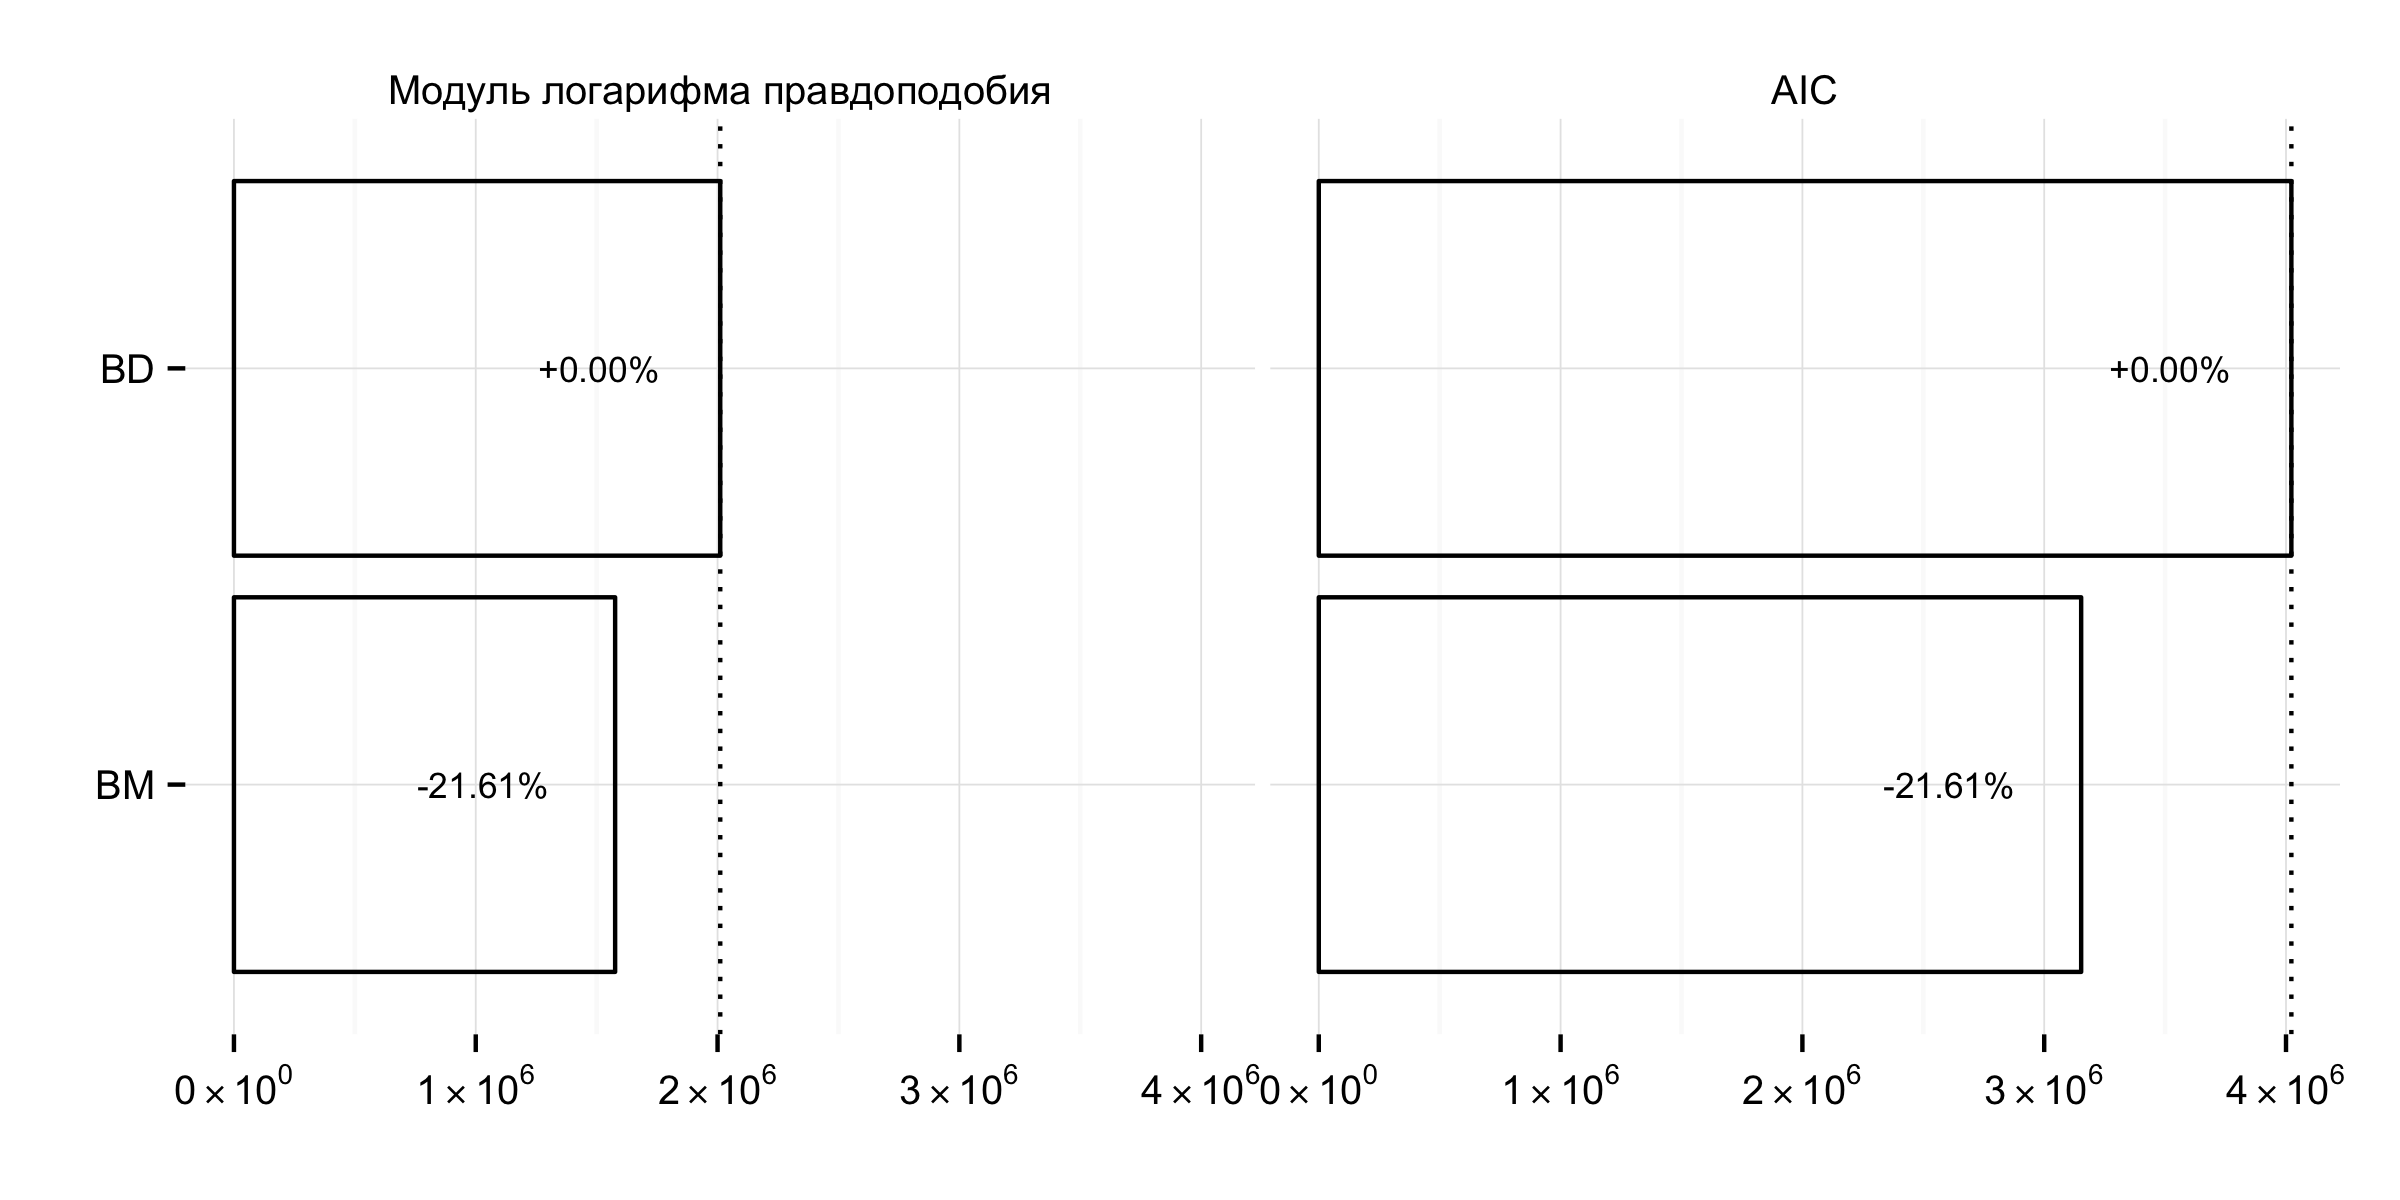
\includegraphics[width=\textwidth]{images/bd-bm}
  \caption{Сравнение одного биномиального распределения (BD) и биномиальной смеси (BM)
    на данных бисульфитного секвенирования стволовых клеток мыши.}
  \label{fig:bd-bm}
\end{figure}


\subsection{Биномиальная скрытая марковская модель}

\subsubsection{Мотивация}

Предположение о независимости состояний соседних цитозинов в геноме выглядит
не очень правдоподобным \cite{Saxonov2006}. Чтобы учесть зависимость состояний двух последовательных
цитозинов, перейдём к биномиальной скрытой марковской модели (СММ) первого порядка.
В СММ состояние $t$-го цитозина зависит только от состояния $(t-1)$-го.

\subsubsection{Определение}

Пусть $\mathbf{\pi} = (\pi_1, \ldots, \pi_S)$ --- вектор априорных
вероятностей состояний, $\mathbf{A}$~---~матрица вероятностей перехода между
состояниями и $\mathbf{p} = (p_1, \ldots, p_S)$ --- параметры биномиального
распределения для каждого из состояний, причём
$$
\sum\limits_{i = 1}^S \pi_i = 1,
\qquad
\forall i \in \{1, \ldots, S\}
\left( \sum\limits_{j = 1}^S \mathbf{A}_{ij} = 1  \right),
$$
тогда функция правдоподобия определяется как
$$
P(\mathbf{k}; \mathbf{n}, \mathbf{\pi}, \mathbf{A}, \mathbf{p})
= \sum\limits_{\mathbf{s} \in \{1, \ldots, S\}^T}
  \pi_{s_1}
  \prod\limits_{t = 2}^T A_{s_t s_{t - 1}}
  \prod\limits_{t = 1}^T \op{Bin}(k_t; n_t, p_{s_t})
$$

Порождающий процесс для биномиальной скрытой марковской модели формулируется
следующим образом: случайно выберем скрытое состояние $s_1$ из дискретного
распределения с параметрами $\mathbf{\pi}$, породим $k_1$ из биномиального
распределения с параметрами $n_1$ и $p_{s_1}$. Выберем следующее состояние
$s_2$ из дискретного распределения $\mathbf{A}_{s_1}$ и продолжим аналогично
(рис.~\ref{fig:generative-hmm}).

\begin{figure}[h]
  \centering
  \begin{tikzpicture}
    \node[latent] (z)  {$s_t$};
    \node[obs, below=of z]    (k)  {$k_t$};
    \node[obs, left=of k]     (n)  {$n_t$};
    \node[latent, right=of k] (p) {$p_i$};
    \node[latent, right=of z] (A) {$\mathbf{A}_i$};

    \edge {z,p,n} {k};

    \node[latent, left=of z] (z0) {$s_{t - 1}$};
    \edge {z0,A} {z};

    \plate {Ap} {(A)(p)} {$S$};
  \end{tikzpicture}
  \caption{Графическая диаграмма для биномиальной СММ}
  \label{fig:generative-hmm}
\end{figure}


\subsubsection{ОМП-вывод}

У задачи ОМП для скрытой марковской модели есть проблемы, аналогичные проблемам описанной ранее
смеси. Найти приближенное решение можно с помощью частного случая EM-алгоритма для скрытых
марковских моделей, традиционно называемого алгоритмом Баума-Велша.

\paragraph{Шаг E}

Шаг E для скрытой марковской модели предполагает вычисление:
\begin{align*}
  \E{\mathbf{s}|\mathbf{k}, \mathbf{n}, \mathbf{\theta^{\op{old}}}}{\I{s_t = i}}
  := \gamma_{ti}
  &= \frac{\alpha_i(t) \beta_i(t)}{\sum\limits_{i' = 1}^S \alpha_{i'}(t) \beta_{i'}(t)} \\
  \E{\mathbf{s}|\mathbf{k}, \mathbf{n}, \mathbf{\theta^{\op{old}}}}{\I{s_t = j} \I{s_{t - 1} = i}}
  := \xi_{tij}
  &= \frac{\alpha_i(t - 1) \mathbf{A}_{ij} \op{Bin}(k_t; n_t, p_j) \beta_j(t)}
          {\sum\limits_{i' = 1}^S \sum\limits_{j' = 1}^S
           \alpha_{i'}(t - 1) \mathbf{A}_{i'j'} \op{Bin}(k_t; n_t, p_{j'}) \beta_{j'}(t)},
\end{align*}
где величины $\alpha_i(t) = P(s_t = i, k_1, \ldots, k_t; \mathbf{\theta})$ и
$\beta_i(t) = P(k_{t + 1}, \ldots, k_T| s_t = i; \mathbf{\theta})$
находятся с помощью алгоритма прямого-обратного хода, который заключается в
динамическом вычислении следующих соотношений (см., например, \cite{Rabiner1989}):
\begin{align*}
  \alpha_i(1)
  &= \pi_i \op{Bin}(k_1; n_1, p_i) \\
  \alpha_i(t)
  &= \left( \sum\limits_{j = 1}^S \alpha_j(t - 1) \mathbf{A}_{ji}
     \right) \op{Bin}(k_t; n_t, p_i) \\
  \beta_i(T)
  &= 1 \\
  \beta_i(t)
  &= \sum\limits_{j = 1}^S \mathbf{A}_{ij} \op{Bin}(k_{t + 1}; n_{t + 1}, p_j) \beta_j(t + 1).
\end{align*}

\paragraph{Шаг M}

Новое приближение параметров находится по формулам:
\begin{align*}
  \pi_i^{\op{new}} &= \gamma_{1i} \\
  \mathbf{A}_{ij}^{\op{new}}
  &= \frac{\sum\limits_{t = 1}^T \xi_{tij}}
          {\sum\limits_{j' = 1}^S\sum\limits_{t = 1}^T \xi_{tij'}} \\
  p_i^{\op{new}}
  &= \frac{\sum\limits_{t = 1}^T \gamma_{ti} k_t}{\sum\limits_{t = 1}^T \gamma_{ti} n_t}
\end{align*}


\paragraph{Алгоритм Витерби}

Для нахождения оценки максимального правдоподобия для последовательности
скрытых состояний модели используется алгоритм Витерби \cite{Rabiner1989}. В процессе работы
алгоритм динамически максимизирует вероятность подпоследовательности
$s_1, \ldots, s_t$ скрытых состояний:
\begin{align*}
  \mathbf{V}_{ti}
  &= \max\limits_{s_1, \ldots, s_{t- 1}} P(s_t = i, s_1, \ldots, s_{t - 1}| \mathbf{k}) \\
  &= \op{Bin}(k_t; n_t, p_i) \left(
         \max\limits_{j = 1}^S \mathbf{V}_{(t - 1)j} \mathbf{A}_{ji}
     \right)
\end{align*}

Наиболее вероятная последовательность состояний может быть найдена
обратным обходом матрицы $\mathbf{V}$, начиная с позиции
$\argmax\limits_{i \in \{1, \ldots, S\}} \mathbf{V}_{T i}$.


\subsubsection{Применение}
\label{bhmm:applications}

Биномиальная скрытая марковская модель обучается на данных бисульфитного секвенирования
первой хромосомы стволовых клеток мыши (см.~\ref{sub:data}). Инициализация параметров модели
производится с помощью биномиальной смеси, обученной на тех же данных. Из графика
(рис.~\ref{fig:bm-bhmm}) можно видеть, что предположение о зависимости состояний последовательных
цитозинов подтвердилось: биномиальная скрытая марковская модель более правдоподобна и имеет
меньшее значение критерия Акаике чем биномиальная смесь.

\begin{figure}[h]
  \centering
  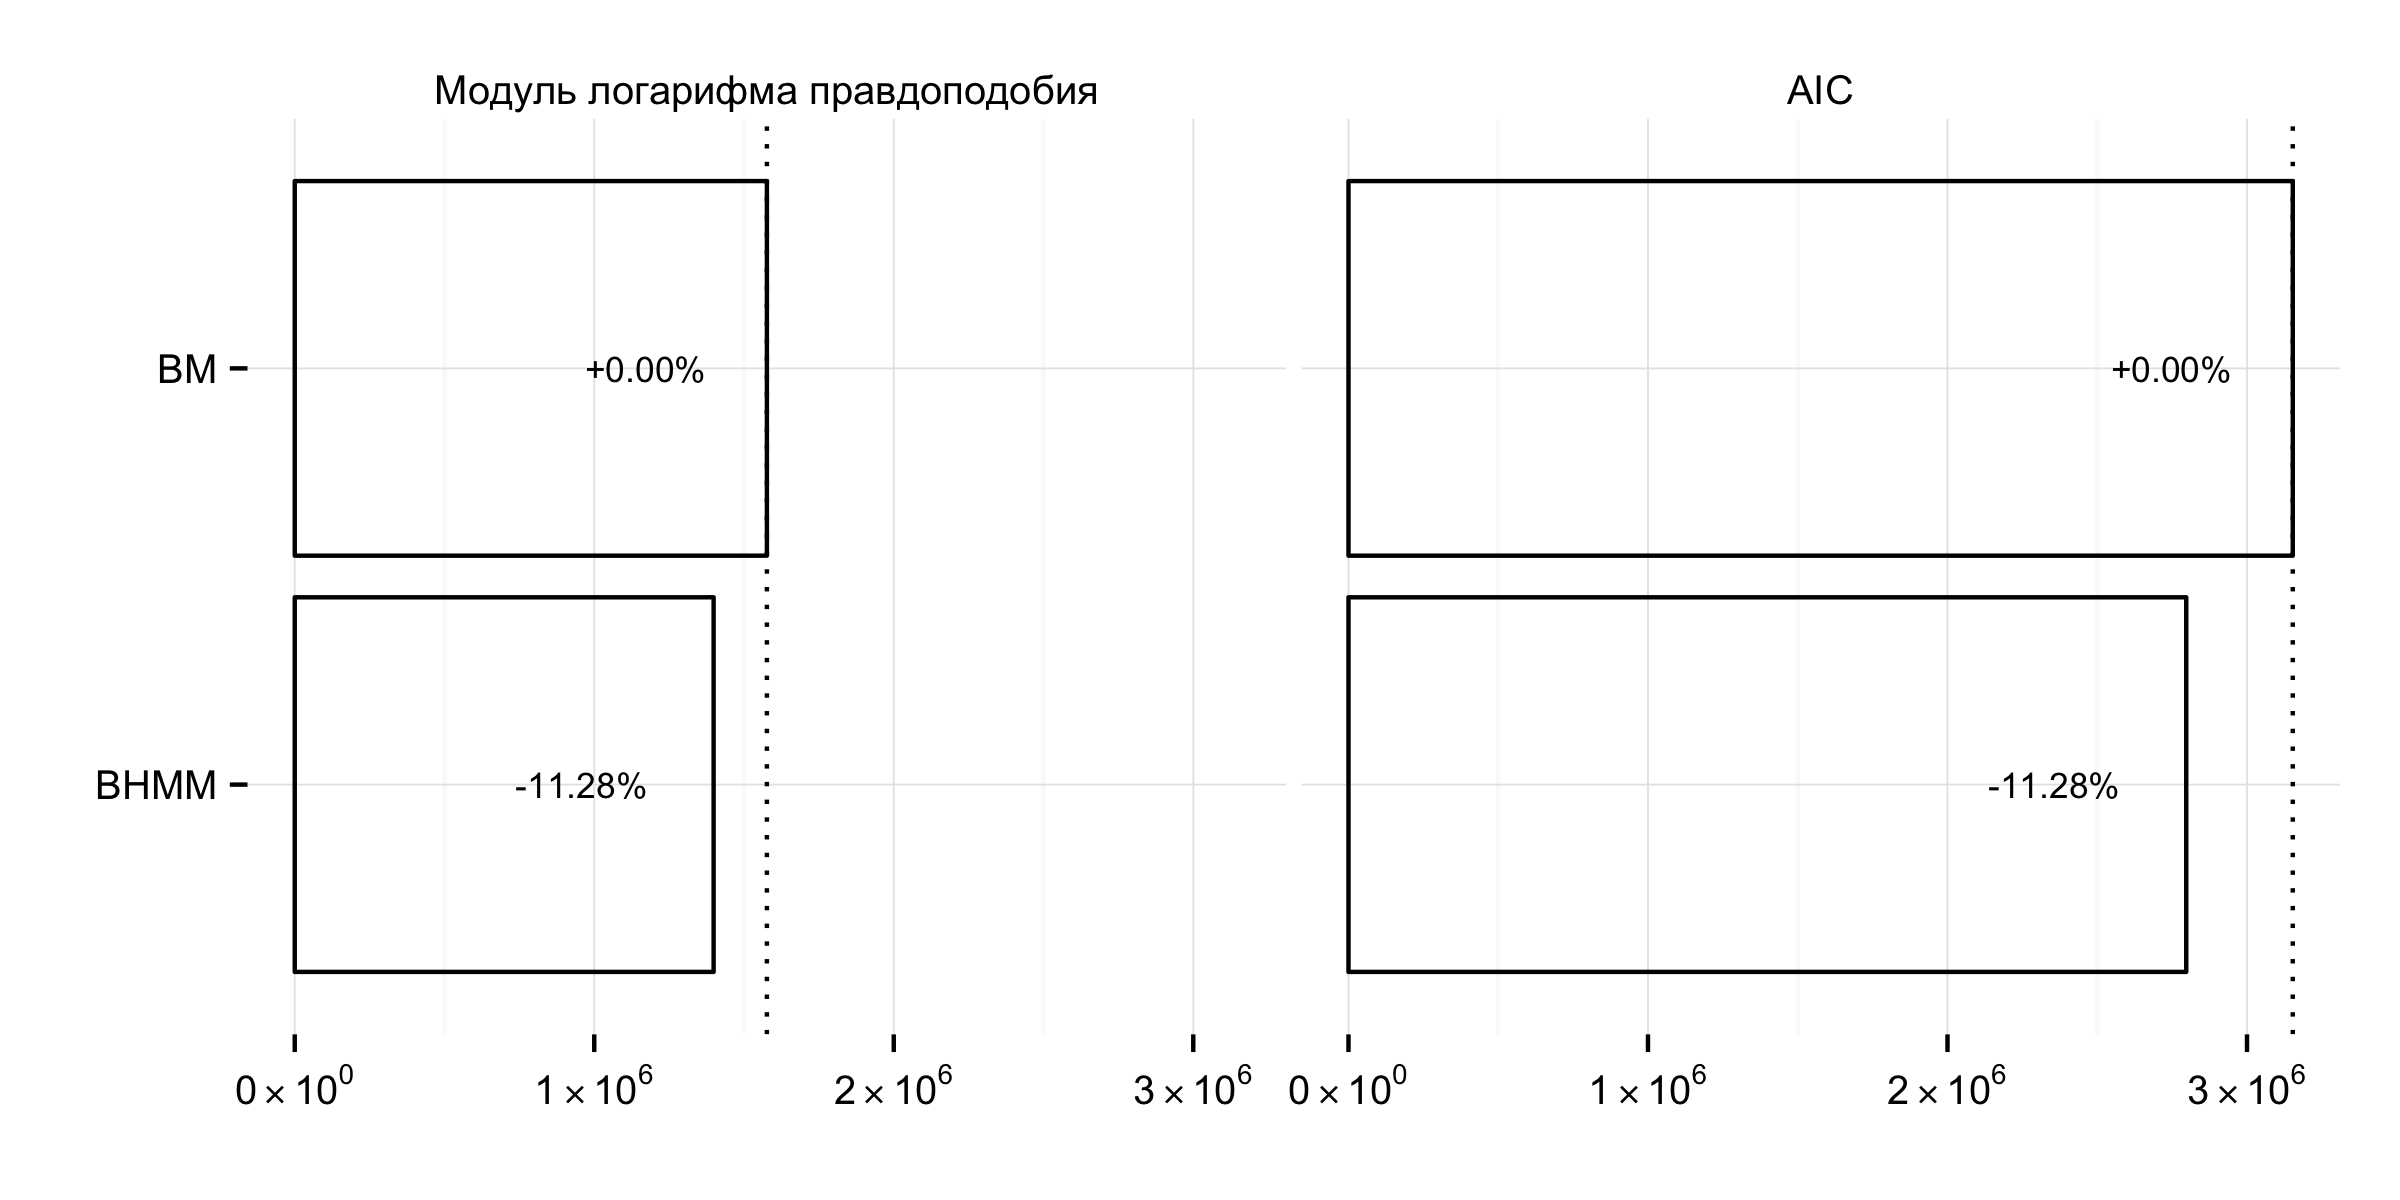
\includegraphics[width=\textwidth]{images/bm-bhmm}
  \caption{Сравнение биномиальной смеси (BM) и биномиальной скрытой марковской модели (BHMM)
    на данных бисульфитного секвенирования стволовых клеток мыши.}
  \label{fig:bm-bhmm}
\end{figure}


\subsection{Переключающаяся биномиальная СММ}

\subsubsection{Мотивация}

Два последовательных цитозина в моделируемых данных в геноме могут находиться
на некотором расстоянии. Предположим, что распределение состояний для следующего
цитозина зависит не только от состояния предыдущего, но также и от расстояния между
ними.

\subsubsection{Определение}

Пусть $d_t$ --- количество нуклеотидов в геноме между $(t-1)$-ым и $t$-ым цитозином,
тогда вероятность перехода из состояния $i$ в состояние $j$ на шаге $t$ можно
определить как
$$
P(s_t = j|s_{t-1} = i, d_t) \propto 1 + \left( \mathbf{A}_{ij} \right)^{d_t}.
$$

К сожалению, при таком определении вероятности перехода получить аналитическое
выражение для $\mathbf{A}_{ij}^{\op{new}}$ не представляется возможным, поэтому
стоит упростить определение, разрешая модели выбирать матрицу вероятностей
перехода в зависимости от расстояния $d_t$:
$$
P(s_t = j|s_{t-1} = i, d_t) = \mathbf{A}_{\op{w}(d_t)ij},
$$
где $\op{w}(d_t) : \mathbb{N}_0 \to \{1, \ldots, D\}$ --- функция,
кластеризующая расстояния. Необходимость в кластеризации расстояний объясняется тем, что
количество различных расстояний в моделируемых данных действительно велико
(рис.~\ref{fig:cytosine-distance}).

\begin{figure}[h!]
  \centering
  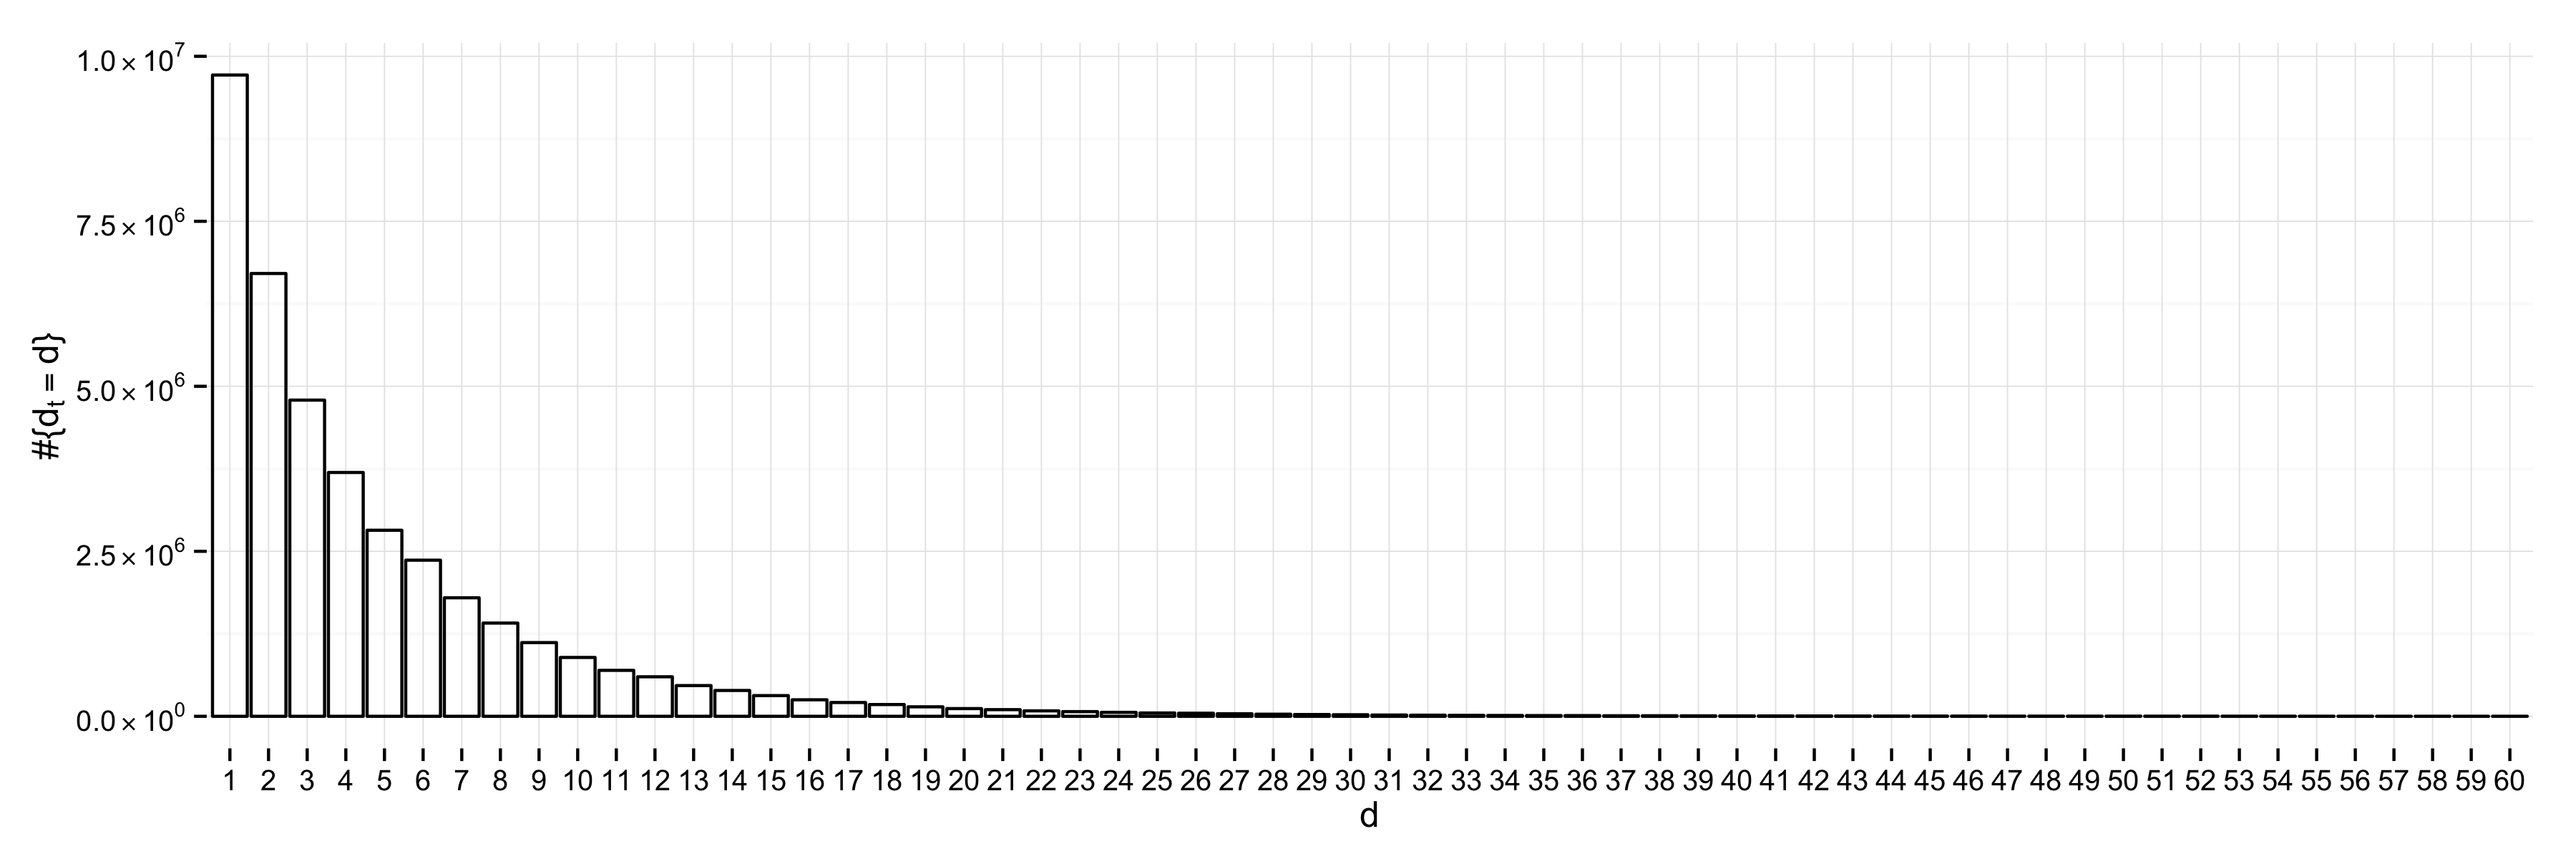
\includegraphics[width=\textwidth]{images/distance_distribution}
  \caption{Гистограмма расстояний между последовательными цитозинами на положительной
    цепи хромосомы 1 генома мыши mm9. Из соображений наглядности на гистограмме изображены
    только расстояния, встречающиеся не менее 1000 раз.}
  \label{fig:cytosine-distance}
\end{figure}

Таким образом, переключающаяся скрытая марковская модель имеет те же параметры, что
и классическая скрытая марковская модель, за исключением матрицы вероятностей перехода
между состояниями модели, которая в случае переключающейся модели индексируется
множеством расстояний $\{1, \ldots, D\}$. Запишем функцию правдоподобия:

$$
P(\mathbf{k}; \mathbf{n}, \mathbf{\pi}, \mathbf{A}, \mathbf{p})
= \sum\limits_{\mathbf{s} \in \{1, \ldots, S\}^T}
  \pi_{s_t}
  \prod\limits_{t = 2}^T A_{\op{w}(d_t) s_t s_{t - 1}}
  \prod\limits_{t = 1}^T \op{Bin}(k_t; n_t, p_{s_t}).
$$

Порождающий процесс для биномиальной переключающейся СММ эквивалентен порождающему
процессу для классической СММ, так как модель не рассматривает расстояния между
наблюдениями как случайную величину.

\subsubsection{Одномерная кластеризация расстояний}

Задача одномерной кластеризации на $D$ классов эквивалентна задаче
разбиения числовой прямой с помощью $D - 1$ разделителей. Существует
несколько подходов к расстановке разделителей, например,

\begin{itemize}
\item в качестве $i$-го разделителя можно взять $^i/_D$-ю
  выборочную квантиль\footnote{Квантилью уровня $\alpha$ распределения
    некоторой случайной величины $X$ называется такое значение $x_{\alpha}$,
    что $P(X \le x_{\alpha}) \ge \alpha$ и $P(X > x_{\alpha}) \le \alpha$.},
  или
\item воспользоваться оптимизацией естественных разделителей
  Дженкса\footnote{\url{http://en.wikipedia.org/wiki/Jenks_natural_breaks_optimization}},
  которая выбирает разделители, минимизирующие дисперсию внутри кластеров
  и максимизирующие дисперсию между кластерами.
\end{itemize}

Оба подхода требуют на вход фиксированное число кластеров и плохо работают
в случае, когда распределение данных имеет тяжелый хвост \cite{jiang2013head}.

Алгоритм <<голова/хвост>> был предложен в качестве альтернативного подхода к
расстановке нефиксированного числа разделителей специально для распределений
с тяжёлым хвостом.

\begin{enumerate}
\item Пусть $\mathbf{d} = (d_1, \ldots, d_T)$ --- вектор расстояний,
  обозначим его среднее за $\overline{d}$ и назовём головой элементы
  $\op{hd}(\mathbf{d}) = (d_t < \overline{d} | t \in \{1, \ldots, T\})$,
  а хвостом $\op{tl}(\mathbf{d}) = (d_t > \overline{d}| t \in \{1, \ldots, T\})$.
\item Добавим $\overline{d}$ во множество разделителей и заменим вектор расстояний
  на голову $\mathbf{d} = \op{hd}(\mathbf{d})$.
\item Если в новом векторе расстояний больше одного элемента, перейдем к шагу 1,
  иначе вернём множество разделителей.
\end{enumerate}

\subsubsection{ОМП-вывод}

ОМП для переключающейся скрытой марковской модели практически полностью
идентична ОМП для классической скрытой марковской модели. Кратко опишем отличающиеся
части шагов E и М.

\paragraph{Шаг E}

Изменим алгоритм прямого-обратного хода для переключающейся скрытой
марковской модели:
\begin{align*}
  \alpha_i(1)
  &= \pi_i \op{Bin}(k_1; n_1, p_i) \\
  \alpha_i(t)
  &= \left( \sum\limits_{j = 1}^S \alpha_j(t - 1) \mathbf{A}_{\op{w}(d_t)ji}
     \right) \op{Bin}(k_t; n_t, p_i) \\
  \beta_i(T)
  &= 1 \\
  \beta_i(t)
  &= \sum\limits_{j = 1}^S
     \mathbf{A}_{\op{w}(d_{t+1})ij} \op{Bin}(k_{t + 1}; n_{t + 1}, p_j) \beta_j(t + 1),
\end{align*}
формулы для вычисления $\gamma_{ti}$ и $\xi_{tij}$ при этом не изменятся.

\paragraph{Шаг М}

Воспользуемся методом множителей Лагранжа для учёта ограничений на матрицу перехода.
Составим функцию Лагранжа
\begin{align*}
  L(\mathbf{\theta}, \mathbf{\Lambda}|\mathbf{\theta}^{\op{old}})
  &= \sum\limits_{t = 2}^T
     \sum\limits_{i = 1}^S \sum\limits_{i = j}^S
     \E{\mathbf{s}|\mathbf{n}, \mathbf{k}, \mathbf{\theta}^{\op{old}}}
       {\I{s_{t - 1} = i}\I{s_t = j}} \log \mathbf{A}_{\op{w}(d_t)ij} \\
  &+ Q(\mathbf{\pi}, \mathbf{p}|\mathbf{\theta}^{\op{old}})
   + \sum\limits_{d = 1}^D \sum\limits_{i = 1}
     \mathbf{\Lambda}_{di} (1 - \sum\limits_{j = 1}^S \mathbf{A}_{dij}),
\end{align*}
где $Q(\mathbf{\pi}, \mathbf{p}|\mathbf{\theta}^{\op{old}})$ --- часть
функции $Q$, не зависящая от $\mathbf{A}$ (см. \cite[c. 620]{murphy2012machine}).

Обозначим
$$
\E{\mathbf{s}|\mathbf{n}, \mathbf{k}, \mathbf{\theta}^{\op{old}}}
  {\I{s_{t - 1} = i}\I{s_t = j}} := \xi_{tij}
$$
и найдём частные производные функции Лагранжа по $\mathbf{A}_{dij}$ и $\mathbf{\Lambda}_{di}$:
\begin{align*}
  \frac{\partial}{\partial \mathbf{A}_{dij}}
  L(\mathbf{\theta}, \mathbf{\Lambda}|\mathbf{\theta}^{\op{old}})
  &= \frac{1}{\mathbf{A}_{dij}} \sum\limits_{t = 2}^T
     \xi_{tij}\I{\op{w}(d_t) = d} - \mathbf{\Lambda}_{di} \equiv 0 \\
  &\Leftrightarrow \mathbf{A}_{dij}
   = \frac{1}{\mathbf{\Lambda}_{di}} \sum\limits_{t = 2}^T
     \xi_{tij} \I{\op{w}(d_t) = d} \\
  \frac{\partial}{\partial \mathbf{\Lambda}_{di}}
  L(\mathbf{\theta}, \mathbf{\Lambda}|\mathbf{\theta}^{\op{old}})
  &= 1 - \sum\limits_{j = 1}^S \mathbf{A}_{dij}
   = 1 -
     \frac{1}{\mathbf{\Lambda}_{di}} \sum\limits_{t = 2}^T
     \sum\limits_{j = 1}^S \xi_{tij} \I{\op{w}(d_t) = d} \equiv 0 \\
  &\Leftrightarrow \mathbf{\Lambda}_{di}
  = \sum\limits_{t = 2}^T
    \sum\limits_{j = 1}^S \xi_{tij} \I{\op{w}(d_t) = d} \\
  &\Rightarrow \mathbf{A}_{dij}^{\op{new}}
  = \frac{\sum\limits_{t = 2}^T \xi_{tij} \I{\op{w}(d_t) = d}}
         {\sum\limits_{j = 1}^S
          \sum\limits_{t = 2}^T \xi_{tij} \I{\op{w}(d_t) = d}}
\end{align*}

\subsubsection{Применение}

Переключающаяся биномиальная СММ обучается на данных бисульфитного секвенирования
первой хромосомы стволовых клеток мыши (см.~\ref{sub:data}). В качестве начального
приближения параметров выбираются параметры биномиальной смеси, обученной на тех же
данных (см.~\ref{bhmm:applications}). Кластеризация расстояний производилась с
помощью алгоритма <<голова/хвост>>. В таблице~\ref{tab:trans} приведены полученные в
результате обучения вероятности перехода для трех кластеров расстояний. Можно заметить,
что в матрицах перехода, соответствующих небольшим расстояниям (кластеры 1, 5),
наибольшие вероятности расположены на главной диагонали. В матрице для удаленных
цитозинов (кластер 9) наблюдается обратная ситуация. То есть близко расположенные
цитозины имеют значительно больший шанс оказаться в одном состоянии, чем удалённые.
Таким образом, предположение о влиянии расстояния между цитозинами на характер зависимости
между их состояниями подтвердилось.

\begin{table}[htbp!]
  \centering
  \begin{subtable}{.3\textwidth}
    \centering
    \begin{tabular}{lll}
      0.990 & 0.002 & 0.008 \\
      0.016 & 0.980 & 0.004 \\
      0.007 & 0.05 & 0.988
    \end{tabular}
    \caption{$\op{w}(d_t) = 1, d_t \in [1, 2]$}
  \end{subtable}\hspace{.025\textwidth}%
  \begin{subtable}{.3\textwidth}
    \centering
    \begin{tabular}{lll}
      0.966 & 0.020 & 0.014 \\
      0.021 & 0.976 & 0.003 \\
      0.006 & 0.007 & 0.987
    \end{tabular}
    \caption{$\op{w}(d_t) = 5, d_t \in [6, 9]$}
  \end{subtable}\hspace{.025\textwidth}%
  \begin{subtable}{.3\textwidth}
    \centering
    \begin{tabular}{lll}
      0.285 & 0.257 & 0.458 \\
      0.056 & 0.413 & 0.531 \\
      0.01  & 0.056 & 0.934
    \end{tabular}
    \caption{$\op{w}(d_t) = 9, d_t \ge 118$}
  \end{subtable}

  \caption{Матрицы вероятностей перехода для переключающейся биномиальной СММ.
    Метки столбцов и строчек слева-направо и сверху вниз: \texttt{UNMETHYLATED},
    \texttt{LOW}, \texttt{HIGH}.}
  \label{tab:trans}
\end{table}

Из графика сравнения классической и переключающейся биномиальной СММ
(рис.~\ref{fig:bhmm-bshmm}) видно, что переход к переключающейся модели улучшил
правдоподобие модели и значение критерия Акаике.

\begin{figure}[htbp!]
  \centering
  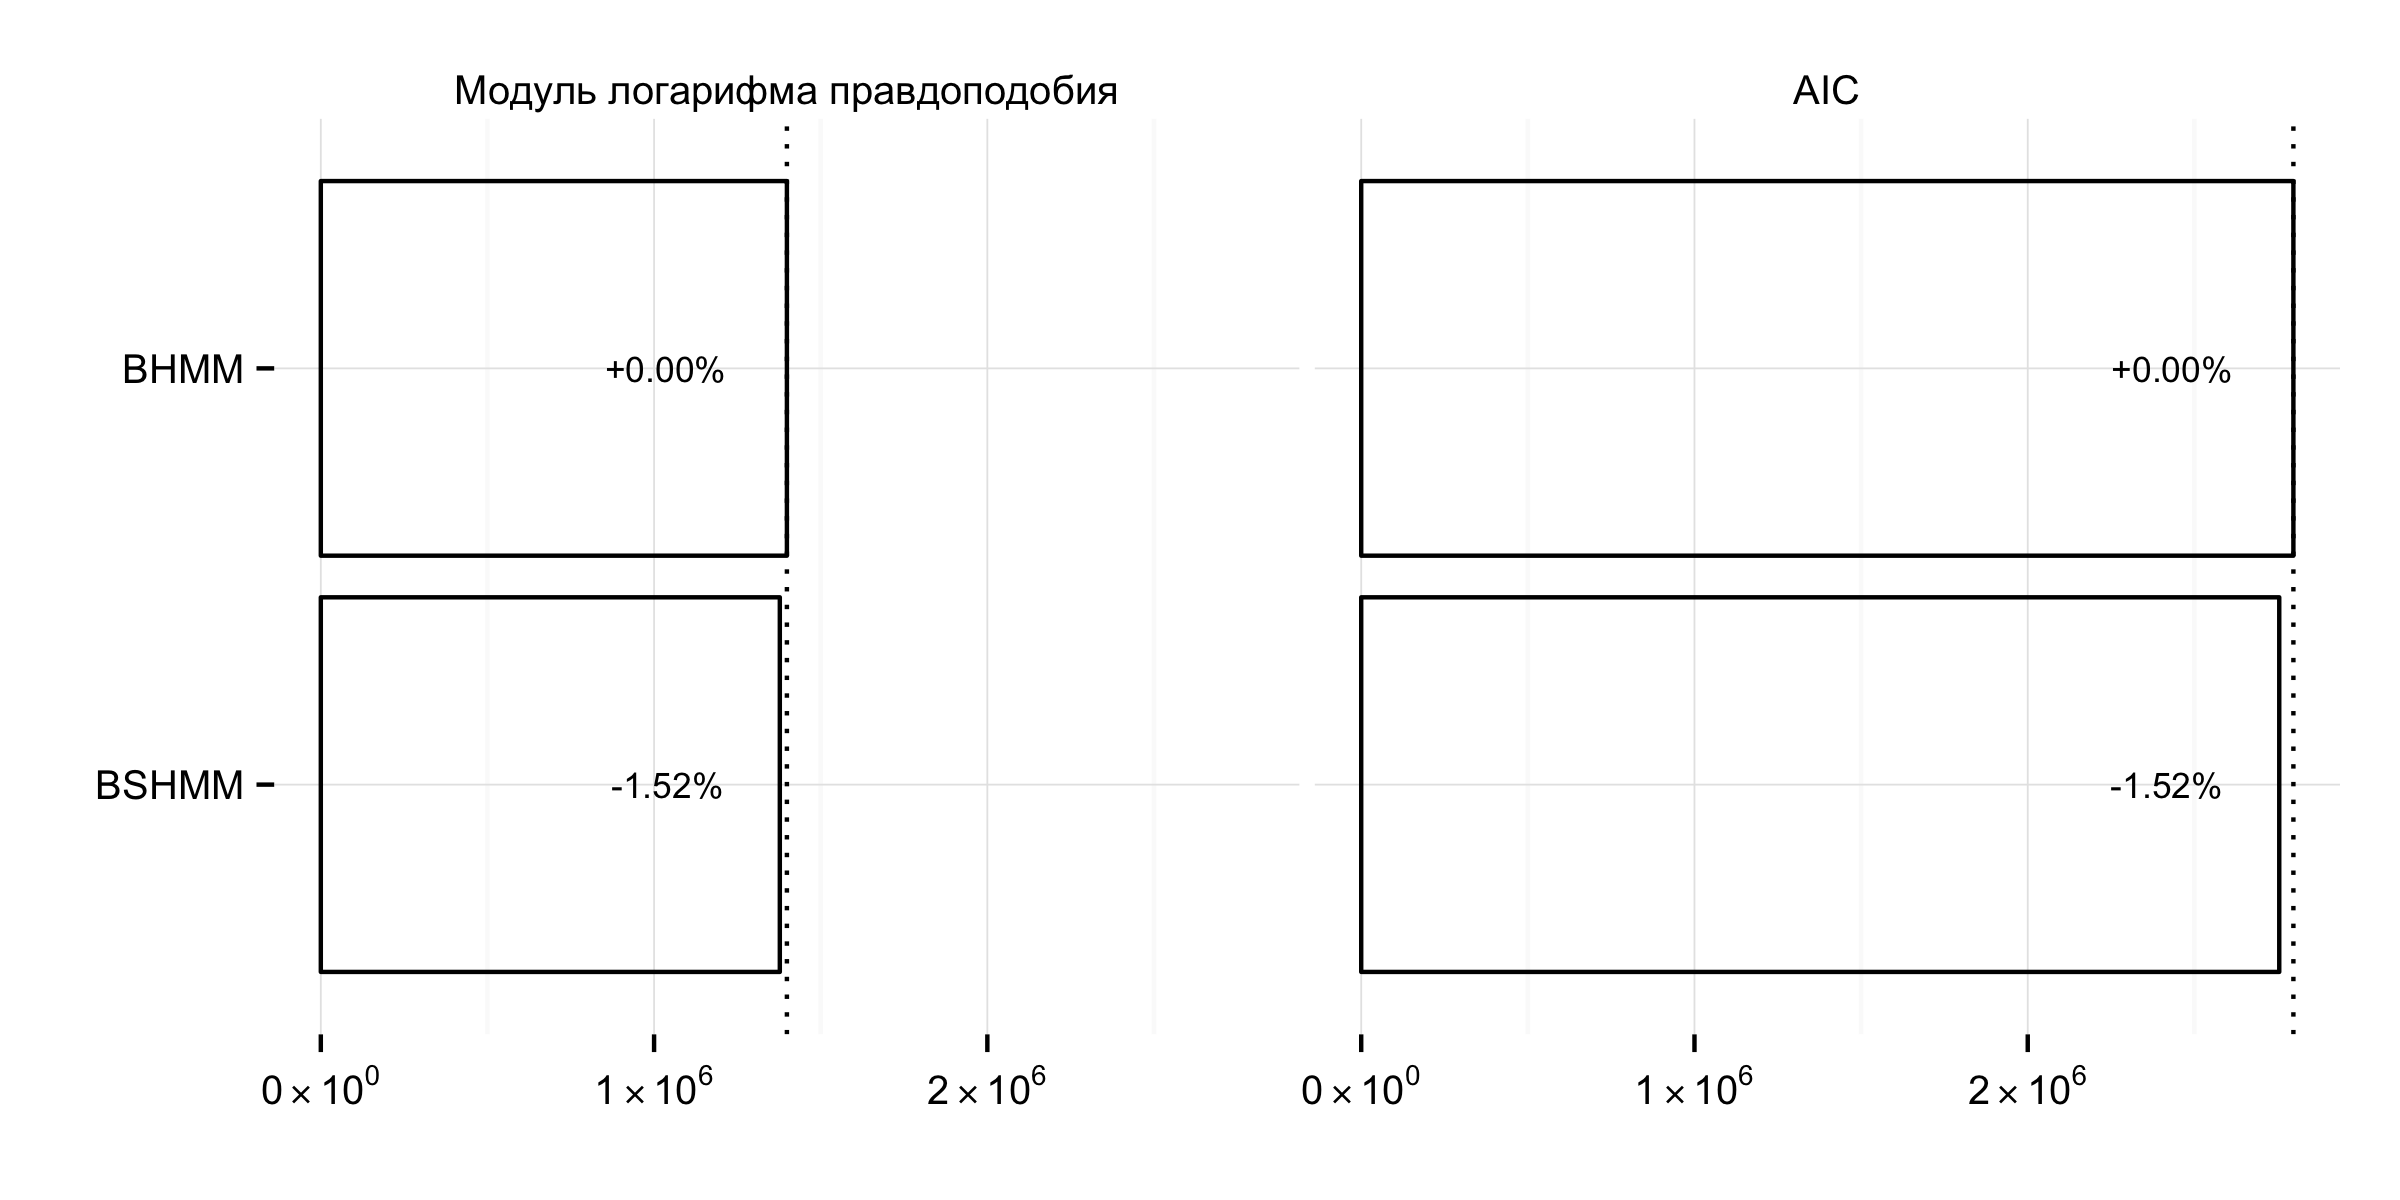
\includegraphics[width=\textwidth]{images/bhmm-bshmm}
  \caption{Сравнение биномиальной классической (BHMM) и переключающейся (BSHMM)
    скрытых марковских моделей на данных бисульфитного секвенирования
    стволовых клеток мыши.}
  \label{fig:bhmm-bshmm}
\end{figure}


\subsection{Переключающаяся мультиномиальная СММ}

\subsubsection{Мотивация}

В предыдущих рассуждениях мы исходили из того, что в прочтениях, полученных
в результате бисульфитного секвенирования, на месте цитозина может быть либо
цитозин, подтверждающий метилирование, либо тимин в обратом случае.
В реальных данных это предположение почти никогда не выполняется, так как
\begin{itemize}
\item в образце могла произойти точечная мутация, в результате которой
  цитозин заменился на другой нуклеотид,
\item секвенаторы делают ошибки при чтении фрагментов \cite{minoche2011evaluation}.
\end{itemize}

Для учёта таких позиций мы будем представлять результаты бисульфитного секвенирования
в виде вектора $x_t = \mathbf{c}_t$, где $c_{t1}$ --- количество прочтений, подтверждающих
аденин в данной позиции, $c_{t2}$ --- цитозин, $c_{t3}$ --- тимин и $c_{t4}$ --- гуанин.
Будем считать, что вектор $\mathbf{c}_t$ подчиняется мультиномиальному распределению с параметрами
$n_t = \sum\limits_{k = 1}^4 c_{tk}$ и $\mathbf{b} = (b_1, \ldots, b_4)$.

\subsubsection{Определение}

Пусть, как и прежде, $\mathbf{\pi}$, $\mathbf{A}$ --- параметры переключающейся
скрытой марковской модели, $\mathbf{B} = (\mathbf{b}_1, \ldots, \mathbf{b}_S)$
--- параметры мультиномиального распределения для каждого из состояний и
$\op{w}$ --- функция, кластеризующая расстояния, тогда функцию правдоподобия можно
записать как
$$
P(\mathbf{k}; \mathbf{n}, \mathbf{\pi}, \mathbf{A}, \mathbf{B})
= \sum\limits_{\mathbf{s} \in \{1, \ldots, S\}^T}
  \pi_{s_t}
  \prod\limits_{t = 2}^T A_{\op{w}(d_t) s_t s_{t - 1}}
  \prod\limits_{t = 1}^T \op{Multin}\left(\mathbf{c}_t; n_t, \mathbf{b}_{s_t}\right).
$$

\subsubsection{ОМП-вывод}

Новое приближение параметров мультиномиального распределение находится по
формулам:
\begin{align*}
  \mathbf{b}^{\op{new}}_{ik}
  = \frac{\sum\limits_{t = 1}^T \gamma_{ti} c_{tk}} {\sum\limits_{t = 1}^T \gamma_{ti} n_t}.
\end{align*}


\subsubsection{Применение}

Переключающаяся мультиномиальная СММ обучается на данных бисульфитного секвенирования
первой хромосомы стволовых клеток мыши (см.~\ref{sub:data}). Начальное приближение
для параметров модели находится с помощью уже упомянутого алгоритма кластеризации
KMeans++ (см.~\ref{bm:applications}). Из графика (рис.~\ref{fig:multinomial}) видно,
что предположение об ошибках секвенатора подтвердилось: в состоянии \texttt{UNMETHYLATED}
вероятности аденина и гуанина отличны от нуля.

%% TODO: объяснить почему мы не можем сравнивать правдоподобие с перелючающейся биномиальной СММ.
%% TODO: написать что-то про перелесть мультиномиальной модели по сравнению с биномиальной
%% в ключе учёта ошибок и потенциала для future work.

\FloatBarrier
\begin{figure}[h]
  \centering
  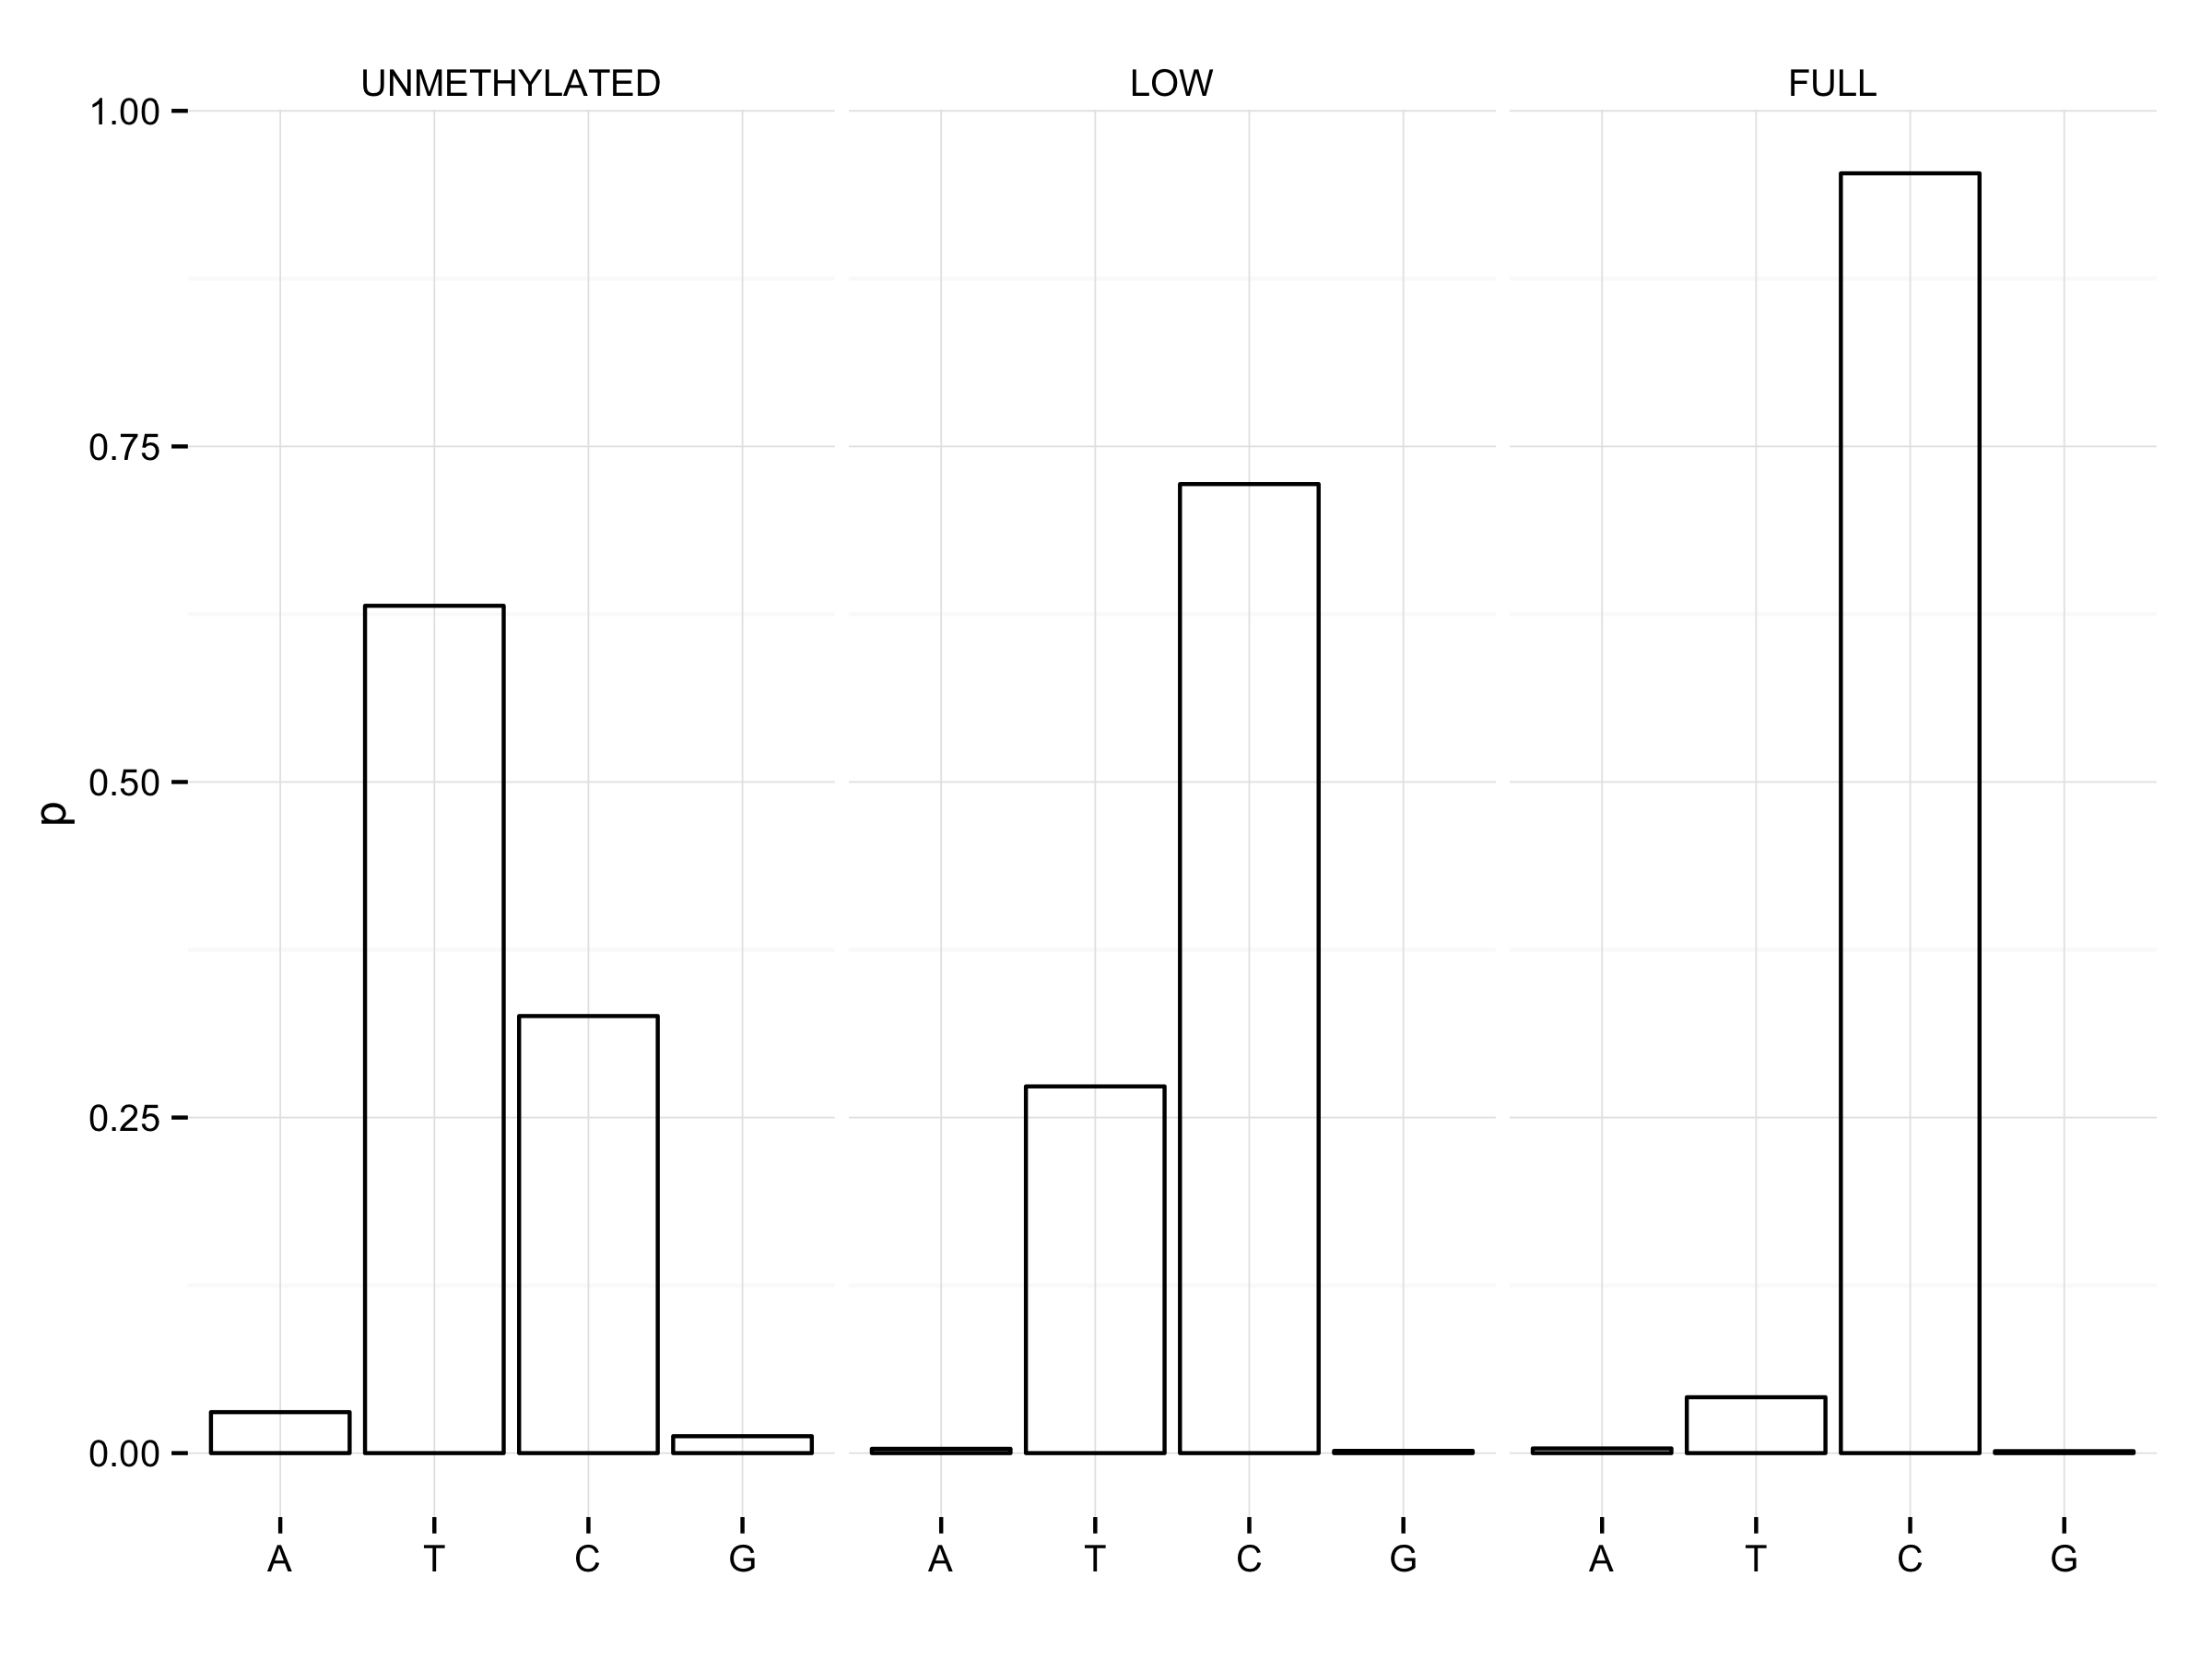
\includegraphics[width=.8\textwidth]{images/multinomial}
  \caption{Распределение нуклеотидов в каждом из состояний модели}
  \label{fig:multinomial}
\end{figure}
\FloatBarrier


\subsection{Программная реализация моделей}
\label{sub:implementation}

Модели были реализованы на языке Java в рамках биоинформатического проекта компании JetBrains.
Оценки времени работы моделей на компьютере с процессором Intel Core i5 1700Mhz и 8Гб оперативной
памяти приведены в таблице~\ref{tab:time}. Можно видеть, что с увеличением сложности модели время
работы увеличивается, но даже для переключающейся мультиномиальной СММ оно не превосходит
25 минут.

\begin{table}[htbp!]
  \centering
  \begin{tabular}{lr}
    \textbf{Модель} & \textbf{Время работы} \\
    \noalign{\nobreak\smallskip}
    Биномиальная смесь & 4 мин. 8 с. \\
    Биномиальная СММ & 6 мин. 55 с. \\
    Переключающаяся биномиальная СММ & 9 мин. 40 с. \\
    Переключающаяся мультиномиальная СММ & 22 мин. 25 с. \\
  \end{tabular}
  \caption{Время работы предлагаемых моделей на данных бисульфитного секвенирования
    первой хромосомы стволовых клеток мыши.}
  \label{tab:time}
\end{table}

%% -*- TeX-engine: xetex; TeX-master: "draft.tex"; ispell-dictionary: "russian" -*-

\section{Количественная оценка модели}

\subsection{Сравнение с существующими моделями}
\label{sub:comparison}

В качестве метода для сравнения мы выбрали  MSC (см.~\ref{subsub:msc}), так как
он ближе всего к предлагаемой модели. Алгоритм MSC использует два состояния, поэтому
мы уменьшили множество состояний переключающейся мультиномиальной СММ до двух, объединив
состояния \texttt{LOW} и \texttt{HIGH} в одно --- \texttt{METHYLATED}.

Результаты работы обоих методов сравнивались на данных бисульфитного секвенирования
стволовых клеток мыши. Допустимое количество ошибок для состояния $\texttt{METHYLATED}$
было ограничено 1\%. Результаты сравнения для трёх первых хромосом генома мыши приведены в
таблице~\ref{table:comparison}. В последней колонке таблицы указано количество метилированных
цитозинов, которые были найдены обеими моделями.
\begin{table}[htbp!]
  \centering
  \begin{tabular}{lrrrr}
    \textbf{Хромосома} & \textbf{MSC} & \textbf{MSHMM} & \textbf{Пересечение} \\
    \noalign{\nobreak\smallskip}
    chr1 & 1136756 & 1291624 & 1136756 \\
    chr2 & 1114488 & 1316179 & 1114488 \\
    chr3 & 896377  & 1040715 & 896377
  \end{tabular}
  \caption{Количество метилированных цитозинов по мнению алгоритма MSC и
    переключающейся мультиномиальной СММ (MSHMM).}
  \label{table:comparison}
\end{table}

\vspace{-7pt}
Получается, что результаты переключающейся мультиномиальной СММ полностью
включают результаты алгоритма MSC, что не удивительно, так как предлагаемая модель
является строгим обобщением биномиальной смеси, используемой в алгоритме MSC.


\subsection{Анализ генов <<домашнего хозяйства>>}
\label{sub:housekeeping}

Гены <<домашнего хозяйства>> (housekeeping genes) --- это гены, необходимые для
поддержания жизнедеятельности клетки в организме. Они активны на всех стадиях
жизненного цикла организма. Одним из необходимых условий активности гена является
отсутствие метилирования в начале гена и в участке до его начала \cite{Jones2012}.

С помощью переключающейся мультиномиальной СММ был проведён анализ метилирования генов
<<домашнего хозяйства>> в мыши (табл.~\ref{tab:housekeeping}). Ожидалось, что у всех
десяти рассматриваемых генов не будет обнаружено метилирование.

\begin{table}[htbp!]
  \centering
  \begin{tabular}{cc}
    \textbf{Идентификатор RefSeq} & \textbf{Символ гена} \\
    \noalign{\nobreak\smallskip}
    NM\_007393 & ACTB \\
    NM\_008951 & PSMD4 \\
    NM\_023372 & RPL38 \\
    NM\_025344 & EIF3F \\
    NM\_026069 & RPL37 \\
    NM\_026885 & CHMP2A \\
    NM\_133691 & PUF60 \\
    NM\_172736 & LENG8 \\
    NM\_172757 & HEATR8 \\
    NM\_198033 & SETX
  \end{tabular}
  \caption{Список генов <<домашнего хозяйства>> в мыши \cite{Kouadjo2007}. Для каждого
    гена приведён соответствующий символ (gene symbol) и идентификатор в базе данных NCBI
    RefSeq.}
  \label{tab:housekeeping}
\end{table}

В результате из десяти генов, у восьми не было отмечено наличие метилирования в начале гена
(рис.~\ref{fig:heatr3}), а два гена начинались с гипометилированного участка (рис.~\ref{fig:setx}).

\begin{figure}[htbp!]
  \centering
  \begin{subfigure}{\textwidth}
    \centering
    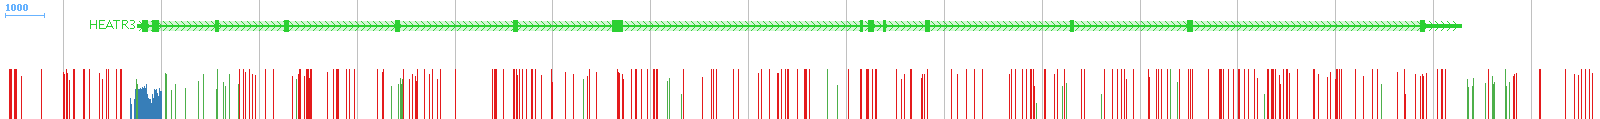
\includegraphics[width=\textwidth]{images/HEATR3}
    \caption{HEATR3}
    \label{fig:heatr3}
  \end{subfigure}
  \par\bigskip
  \begin{subfigure}{\textwidth}
    \centering
    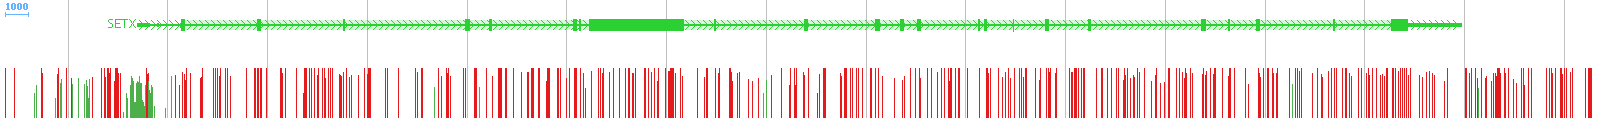
\includegraphics[width=\textwidth]{images/SETX}
    \caption{SETX}
    \label{fig:setx}
  \end{subfigure}
  \caption{Результаты работы переключающейся мультиномиальной СММ на генах <<домашнего хозяйства>> мыши.}
\end{figure}

На основании проведённых экспериментов можно предполагать, что полученная модель биологически
интерпретируема: на восьми из десяти рассмотренных генов <<домашнего хозяйства>> мыши модель
показала результаты, которые соответствуют описанным ожиданиям.

%% -*- TeX-engine: xetex; TeX-master: "draft.tex"; ispell-dictionary: "russian" -*-

\section*{Заключение}

В ходе проделанной работы достигнуты следующие результаты.

\begin{enumerate}
\item Проанализированы и описаны существующие подходы к обработке и моделированию данных бисульфитного
  секвенирования: скрытая марковская модель с Гауссовыми испусканиями, MethylSeekR и MSC.
  (См.~\ref{sub:existing})
\item Разработаны несколько вероятностных моделей: биномиальная смесь, биномиальная скрытая
  марковская модель, переключающаяся биномиальная скрытая марковская модель, переключающаяся
  мультиномиальная скрытая марковская модель. Для каждой модели приведены мотивация, описание и
  обоснование. (См.~\ref{sec:models})
\item В качестве наиболее подходящей модели выбрана переключающаяся мультиномиальная скрытая марковская
  модель, так как она позволяет учитывать особенности моделируемых данных и показала хорошее время
  обучения: 22 минуты на самой большой хромосоме генома мыши. (См.~\ref{sub:implementation})
\item Проведено сравнение переключающейся мультиномиальной скрытой марковской модели с алгоритмом MSC на
  данных бисульфитного секвенирования стволовых клеток мыши. Разработанная модель учла 100\%
  результатов, показанных MSC, а также нашла другие метилированные цитозины.
  (См.~\ref{sub:comparison})
\item Продемонстирована работа модели на генах <<домашнего хозяйства>> мыши. На восьми из десяти
  генов модель показала ожидаемые результаты. (См.~\ref{sub:housekeeping})
\end{enumerate}

В качестве развития модели предполагается учёт точечных мутаций в исследуемых образцах. Кроме того,
планируется обобщение на сравнение нескольких биологических образцов для исследования изменений
метилирования, например, при раке или дифференцировке клетки. Описанную модель также можно расширить
для учёта асимметрии в метилировании соседних цитозинов на разных цепочках ДНК.

Полученная модель уже используется в биоинформатическом проекте компании JetBrains для разметки геномов в
соответствии с уровнем метилирования. Также результаты, описанные в работе, будут оформлены в
статью.


\printbibliography

\end{document}
